\documentclass[letterpaper, 12pt]{article}

\usepackage{amsmath, amsthm, amssymb, dsfont, accents}
\usepackage{hyperref, subcaption, booktabs}
\usepackage{fullpage}

\usepackage{tikz, pgfplots}
\pgfplotsset{compat=newest}
\newlength{\figurewidth}
\newlength{\figureheight}

\newcommand{\argmin}{\operatornamewithlimits{arg\ min}}
\newcommand{\argmax}{\operatornamewithlimits{arg\ max}}
\newcommand{\ind}[1]{\mathds{1}_{{#1}}} 
\newcommand{\ubar}[1]{\underaccent{\bar}{#1}}

\title{4D lane keepin}
\author{Petter Nilsson \\ \href{mailto:pettni@umich.edu}{pettni@umich.edu}}

\begin{document}

\begin{figure}

\setlength\figurewidth{0.4\columnwidth} 
\setlength\figureheight{0.4 \columnwidth} 
		
\begin{subfigure}{0.45\columnwidth}
	% This file was created by matlab2tikz v0.4.7 running on MATLAB 8.2.
% Copyright (c) 2008--2014, Nico Schlömer <nico.schloemer@gmail.com>
% All rights reserved.
% Minimal pgfplots version: 1.3
% 
\begin{tikzpicture}

\begin{axis}[%
width=\figurewidth,
height=\figureheight,
view={-37.5}{30},
scale only axis,
xmin=-1.1,
xmax=1.1,
xlabel={$v$},
xmajorgrids,
ymin=-0.135743544725286,
ymax=0.135743544725286,
ylabel={$\psi$},
ymajorgrids,
zmin=-0.439864664342193,
zmax=0.439864664342193,
zlabel={$r$},
zmajorgrids,
axis x line*=bottom,
axis y line*=left,
axis z line*=left
]

\addplot3[area legend,solid,line width=1.0pt,fill=red,opacity=5.000000e-01,draw=black,forget plot]
table[row sep=crcr] {%
x	y	z\\
1	-0.0438031428676238	-0.282463788556039\\
1	-0.045719488167792	-0.282441205319777\\
1	-0.0606954882711895	-0.281738128304401\\
1	-0.0855267122253757	-0.275029161983213\\
1	-0.119261287753917	-0.211010244973643\\
1	-0.123403222477533	0.364296046889597\\
1	-0.123383668678566	0.399876967583812\\
1	0.0897098665283678	0.399876967583812\\
1	0.0906492132680411	0.269399567101864\\
1	0.0904549793741083	-0.0840366520101617\\
1	0.0862791174032042	-0.282537664938402\\
1	-0.00298309809448049	-0.282537664938402\\
};


\addplot3[area legend,solid,line width=1.0pt,fill=red,opacity=5.000000e-01,draw=black,forget plot]
table[row sep=crcr] {%
x	y	z\\
1	-0.123383668678566	0.399876967583812\\
-0.00317973298121733	-0.106779909477179	0.399876967583812\\
-0.629666672595915	-0.0923440680113889	0.399876967583812\\
-0.629666672595915	-0.00234474831953499	0.399876967583812\\
-0.629438489376948	0.0376006333069677	0.399876967583812\\
-0.629362237417582	0.0396495518232928	0.399876967583812\\
-0.627143263513224	0.0545892117808404	0.399876967583812\\
-0.605969166129405	0.0790736674446303	0.399876967583812\\
-0.403919741780704	0.109499278620261	0.399876967583812\\
-0.40380997302597	0.10949785998026	0.399876967583812\\
1	0.0897098665283678	0.399876967583812\\
1	0.0897098665283678	0.399876967583812\\
};


\addplot3[area legend,solid,line width=1.0pt,fill=red,opacity=5.000000e-01,draw=black,forget plot]
table[row sep=crcr] {%
x	y	z\\
-1	0.00298309809041029	0.282537664938406\\
-1	-0.0862791174032011	0.282537664938406\\
-1	-0.0904549793741084	0.0840366520100114\\
-1	-0.0906492132680412	-0.269399567101865\\
-1	-0.0897098665283678	-0.399876967583812\\
-1	0.123383668678566	-0.399876967583812\\
-1	0.123403222477533	-0.364296046889598\\
-1	0.119261287753917	0.211010244973579\\
-1	0.0855267122253341	0.275029161983228\\
-1	0.0606954882711949	0.281738128304402\\
-1	0.045719488167792	0.282441205319779\\
-1	0.0438031428681564	0.282463788556035\\
};


\addplot3[area legend,solid,line width=1.0pt,fill=red,opacity=5.000000e-01,draw=black,forget plot]
table[row sep=crcr] {%
x	y	z\\
-1	-0.0897098665283678	-0.399876967583812\\
0.403809973026625	-0.109497859980269	-0.399876967583812\\
0.403919741780907	-0.109499278620265	-0.399876967583812\\
0.605969166129359	-0.0790736674446712	-0.399876967583812\\
0.627143263513218	-0.054589211780835	-0.399876967583812\\
0.629362237417575	-0.0396495518232929	-0.399876967583812\\
0.629438489376961	-0.0376006333064349	-0.399876967583812\\
0.629666672595902	0.0023447483154774	-0.399876967583812\\
0.629666672595902	0.0923440680113922	-0.399876967583812\\
0.00317973298169149	0.106779909477171	-0.399876967583812\\
-1	0.123383668678566	-0.399876967583812\\
-1	0.123383668678566	-0.399876967583812\\
};


\addplot3[area legend,solid,line width=1.0pt,fill=red,opacity=5.000000e-01,draw=black,forget plot]
table[row sep=crcr] {%
x	y	z\\
-0.629362237417582	0.0396495518232928	0.399876967583812\\
-0.629438489376948	0.0376006333069677	0.399876967583812\\
-1	0.0438031428681564	0.282463788556035\\
-1	0.045719488167792	0.282441205319779\\
-1	0.045719488167792	0.282441205319779\\
-1	0.045719488167792	0.282441205319779\\
-1	0.045719488167792	0.282441205319779\\
-1	0.045719488167792	0.282441205319779\\
-1	0.045719488167792	0.282441205319779\\
-1	0.045719488167792	0.282441205319779\\
-1	0.045719488167792	0.282441205319779\\
-1	0.045719488167792	0.282441205319779\\
};


\addplot3[area legend,solid,line width=1.0pt,fill=red,opacity=5.000000e-01,draw=black,forget plot]
table[row sep=crcr] {%
x	y	z\\
1	0.0906492132680411	0.269399567101864\\
1	0.0897098665283678	0.399876967583812\\
-0.40380997302597	0.10949785998026	0.399876967583812\\
-1	0.123403222477533	-0.364296046889598\\
-1	0.123403222477533	-0.364296046889598\\
-1	0.123403222477533	-0.364296046889598\\
-1	0.123403222477533	-0.364296046889598\\
-1	0.123403222477533	-0.364296046889598\\
-1	0.123403222477533	-0.364296046889598\\
-1	0.123403222477533	-0.364296046889598\\
-1	0.123403222477533	-0.364296046889598\\
-1	0.123403222477533	-0.364296046889598\\
};


\addplot3[area legend,solid,line width=1.0pt,fill=red,opacity=5.000000e-01,draw=black,forget plot]
table[row sep=crcr] {%
x	y	z\\
1	0.0862791174032042	-0.282537664938402\\
1	0.0904549793741083	-0.0840366520101617\\
0.00317973298169149	0.106779909477171	-0.399876967583812\\
0.629666672595902	0.0923440680113922	-0.399876967583812\\
0.629666672595902	0.0923440680113922	-0.399876967583812\\
0.629666672595902	0.0923440680113922	-0.399876967583812\\
0.629666672595902	0.0923440680113922	-0.399876967583812\\
0.629666672595902	0.0923440680113922	-0.399876967583812\\
0.629666672595902	0.0923440680113922	-0.399876967583812\\
0.629666672595902	0.0923440680113922	-0.399876967583812\\
0.629666672595902	0.0923440680113922	-0.399876967583812\\
0.629666672595902	0.0923440680113922	-0.399876967583812\\
};


\addplot3[area legend,solid,line width=1.0pt,fill=red,opacity=5.000000e-01,draw=black,forget plot]
table[row sep=crcr] {%
x	y	z\\
0.00317973298169149	0.106779909477171	-0.399876967583812\\
1	0.0904549793741083	-0.0840366520101617\\
1	0.0906492132680411	0.269399567101864\\
-1	0.123403222477533	-0.364296046889598\\
-1	0.123383668678566	-0.399876967583812\\
-1	0.123383668678566	-0.399876967583812\\
-1	0.123383668678566	-0.399876967583812\\
-1	0.123383668678566	-0.399876967583812\\
-1	0.123383668678566	-0.399876967583812\\
-1	0.123383668678566	-0.399876967583812\\
-1	0.123383668678566	-0.399876967583812\\
-1	0.123383668678566	-0.399876967583812\\
};


\addplot3[area legend,solid,line width=1.0pt,fill=red,opacity=5.000000e-01,draw=black,forget plot]
table[row sep=crcr] {%
x	y	z\\
-1	0.0606954882711949	0.281738128304402\\
-1	0.0855267122253341	0.275029161983228\\
-0.605969166129405	0.0790736674446303	0.399876967583812\\
-0.627143263513224	0.0545892117808404	0.399876967583812\\
-0.627143263513224	0.0545892117808404	0.399876967583812\\
-0.627143263513224	0.0545892117808404	0.399876967583812\\
-0.627143263513224	0.0545892117808404	0.399876967583812\\
-0.627143263513224	0.0545892117808404	0.399876967583812\\
-0.627143263513224	0.0545892117808404	0.399876967583812\\
-0.627143263513224	0.0545892117808404	0.399876967583812\\
-0.627143263513224	0.0545892117808404	0.399876967583812\\
-0.627143263513224	0.0545892117808404	0.399876967583812\\
};


\addplot3[area legend,solid,line width=1.0pt,fill=red,opacity=5.000000e-01,draw=black,forget plot]
table[row sep=crcr] {%
x	y	z\\
-0.40380997302597	0.10949785998026	0.399876967583812\\
-0.403919741780704	0.109499278620261	0.399876967583812\\
-1	0.119261287753917	0.211010244973579\\
-1	0.119261287753917	0.211010244973579\\
-1	0.119261287753917	0.211010244973579\\
-1	0.119261287753917	0.211010244973579\\
-1	0.119261287753917	0.211010244973579\\
-1	0.119261287753917	0.211010244973579\\
-1	0.119261287753917	0.211010244973579\\
-1	0.119261287753917	0.211010244973579\\
-1	0.119261287753917	0.211010244973579\\
-1	0.119261287753917	0.211010244973579\\
};


\addplot3[area legend,solid,line width=1.0pt,fill=red,opacity=5.000000e-01,draw=black,forget plot]
table[row sep=crcr] {%
x	y	z\\
-1	0.0855267122253341	0.275029161983228\\
-1	0.119261287753917	0.211010244973579\\
-0.403919741780704	0.109499278620261	0.399876967583812\\
-0.605969166129405	0.0790736674446303	0.399876967583812\\
-0.605969166129405	0.0790736674446303	0.399876967583812\\
-0.605969166129405	0.0790736674446303	0.399876967583812\\
-0.605969166129405	0.0790736674446303	0.399876967583812\\
-0.605969166129405	0.0790736674446303	0.399876967583812\\
-0.605969166129405	0.0790736674446303	0.399876967583812\\
-0.605969166129405	0.0790736674446303	0.399876967583812\\
-0.605969166129405	0.0790736674446303	0.399876967583812\\
-0.605969166129405	0.0790736674446303	0.399876967583812\\
};


\addplot3[area legend,solid,line width=1.0pt,fill=red,opacity=5.000000e-01,draw=black,forget plot]
table[row sep=crcr] {%
x	y	z\\
-0.629362237417582	0.0396495518232928	0.399876967583812\\
-1	0.045719488167792	0.282441205319779\\
-1	0.0606954882711949	0.281738128304402\\
-0.627143263513224	0.0545892117808404	0.399876967583812\\
-0.627143263513224	0.0545892117808404	0.399876967583812\\
-0.627143263513224	0.0545892117808404	0.399876967583812\\
-0.627143263513224	0.0545892117808404	0.399876967583812\\
-0.627143263513224	0.0545892117808404	0.399876967583812\\
-0.627143263513224	0.0545892117808404	0.399876967583812\\
-0.627143263513224	0.0545892117808404	0.399876967583812\\
-0.627143263513224	0.0545892117808404	0.399876967583812\\
-0.627143263513224	0.0545892117808404	0.399876967583812\\
};


\addplot3[area legend,solid,line width=1.0pt,fill=red,opacity=5.000000e-01,draw=black,forget plot]
table[row sep=crcr] {%
x	y	z\\
-0.629666672595915	-0.00234474831953499	0.399876967583812\\
-1	0.00298309809041029	0.282537664938406\\
-1	0.0438031428681564	0.282463788556035\\
-0.629438489376948	0.0376006333069677	0.399876967583812\\
-0.629438489376948	0.0376006333069677	0.399876967583812\\
-0.629438489376948	0.0376006333069677	0.399876967583812\\
-0.629438489376948	0.0376006333069677	0.399876967583812\\
-0.629438489376948	0.0376006333069677	0.399876967583812\\
-0.629438489376948	0.0376006333069677	0.399876967583812\\
-0.629438489376948	0.0376006333069677	0.399876967583812\\
-0.629438489376948	0.0376006333069677	0.399876967583812\\
-0.629438489376948	0.0376006333069677	0.399876967583812\\
};


\addplot3[area legend,solid,line width=1.0pt,fill=red,opacity=5.000000e-01,draw=black,forget plot]
table[row sep=crcr] {%
x	y	z\\
-0.629666672595915	-0.0923440680113889	0.399876967583812\\
-0.00317973298121733	-0.106779909477179	0.399876967583812\\
-1	-0.0904549793741084	0.0840366520100114\\
-1	-0.0862791174032011	0.282537664938406\\
-1	-0.0862791174032011	0.282537664938406\\
-1	-0.0862791174032011	0.282537664938406\\
-1	-0.0862791174032011	0.282537664938406\\
-1	-0.0862791174032011	0.282537664938406\\
-1	-0.0862791174032011	0.282537664938406\\
-1	-0.0862791174032011	0.282537664938406\\
-1	-0.0862791174032011	0.282537664938406\\
-1	-0.0862791174032011	0.282537664938406\\
};


\addplot3[area legend,solid,line width=1.0pt,fill=red,opacity=5.000000e-01,draw=black,forget plot]
table[row sep=crcr] {%
x	y	z\\
-0.629666672595915	-0.0923440680113889	0.399876967583812\\
-1	-0.0862791174032011	0.282537664938406\\
-1	0.00298309809041029	0.282537664938406\\
-0.629666672595915	-0.00234474831953499	0.399876967583812\\
-0.629666672595915	-0.00234474831953499	0.399876967583812\\
-0.629666672595915	-0.00234474831953499	0.399876967583812\\
-0.629666672595915	-0.00234474831953499	0.399876967583812\\
-0.629666672595915	-0.00234474831953499	0.399876967583812\\
-0.629666672595915	-0.00234474831953499	0.399876967583812\\
-0.629666672595915	-0.00234474831953499	0.399876967583812\\
-0.629666672595915	-0.00234474831953499	0.399876967583812\\
-0.629666672595915	-0.00234474831953499	0.399876967583812\\
};


\addplot3[area legend,solid,line width=1.0pt,fill=red,opacity=5.000000e-01,draw=black,forget plot]
table[row sep=crcr] {%
x	y	z\\
1	-0.123403222477533	0.364296046889597\\
0.403809973026625	-0.109497859980269	-0.399876967583812\\
-1	-0.0897098665283678	-0.399876967583812\\
-1	-0.0906492132680412	-0.269399567101865\\
-1	-0.0906492132680412	-0.269399567101865\\
-1	-0.0906492132680412	-0.269399567101865\\
-1	-0.0906492132680412	-0.269399567101865\\
-1	-0.0906492132680412	-0.269399567101865\\
-1	-0.0906492132680412	-0.269399567101865\\
-1	-0.0906492132680412	-0.269399567101865\\
-1	-0.0906492132680412	-0.269399567101865\\
-1	-0.0906492132680412	-0.269399567101865\\
};


\addplot3[area legend,solid,line width=1.0pt,fill=red,opacity=5.000000e-01,draw=black,forget plot]
table[row sep=crcr] {%
x	y	z\\
1	-0.119261287753917	-0.211010244973643\\
0.403919741780907	-0.109499278620265	-0.399876967583812\\
0.403809973026625	-0.109497859980269	-0.399876967583812\\
0.403809973026625	-0.109497859980269	-0.399876967583812\\
0.403809973026625	-0.109497859980269	-0.399876967583812\\
0.403809973026625	-0.109497859980269	-0.399876967583812\\
0.403809973026625	-0.109497859980269	-0.399876967583812\\
0.403809973026625	-0.109497859980269	-0.399876967583812\\
0.403809973026625	-0.109497859980269	-0.399876967583812\\
0.403809973026625	-0.109497859980269	-0.399876967583812\\
0.403809973026625	-0.109497859980269	-0.399876967583812\\
0.403809973026625	-0.109497859980269	-0.399876967583812\\
};


\addplot3[area legend,solid,line width=1.0pt,fill=red,opacity=5.000000e-01,draw=black,forget plot]
table[row sep=crcr] {%
x	y	z\\
1	-0.123383668678566	0.399876967583812\\
1	-0.123403222477533	0.364296046889597\\
-1	-0.0906492132680412	-0.269399567101865\\
-1	-0.0904549793741084	0.0840366520100114\\
-0.00317973298121733	-0.106779909477179	0.399876967583812\\
-0.00317973298121733	-0.106779909477179	0.399876967583812\\
-0.00317973298121733	-0.106779909477179	0.399876967583812\\
-0.00317973298121733	-0.106779909477179	0.399876967583812\\
-0.00317973298121733	-0.106779909477179	0.399876967583812\\
-0.00317973298121733	-0.106779909477179	0.399876967583812\\
-0.00317973298121733	-0.106779909477179	0.399876967583812\\
-0.00317973298121733	-0.106779909477179	0.399876967583812\\
};


\addplot3[area legend,solid,line width=1.0pt,fill=red,opacity=5.000000e-01,draw=black,forget plot]
table[row sep=crcr] {%
x	y	z\\
0.627143263513218	-0.054589211780835	-0.399876967583812\\
0.605969166129359	-0.0790736674446712	-0.399876967583812\\
1	-0.0855267122253757	-0.275029161983213\\
1	-0.0606954882711895	-0.281738128304401\\
1	-0.0606954882711895	-0.281738128304401\\
1	-0.0606954882711895	-0.281738128304401\\
1	-0.0606954882711895	-0.281738128304401\\
1	-0.0606954882711895	-0.281738128304401\\
1	-0.0606954882711895	-0.281738128304401\\
1	-0.0606954882711895	-0.281738128304401\\
1	-0.0606954882711895	-0.281738128304401\\
1	-0.0606954882711895	-0.281738128304401\\
};


\addplot3[area legend,solid,line width=1.0pt,fill=red,opacity=5.000000e-01,draw=black,forget plot]
table[row sep=crcr] {%
x	y	z\\
1	-0.045719488167792	-0.282441205319777\\
1	-0.0438031428676238	-0.282463788556039\\
0.629438489376961	-0.0376006333064349	-0.399876967583812\\
0.629362237417575	-0.0396495518232929	-0.399876967583812\\
0.629362237417575	-0.0396495518232929	-0.399876967583812\\
0.629362237417575	-0.0396495518232929	-0.399876967583812\\
0.629362237417575	-0.0396495518232929	-0.399876967583812\\
0.629362237417575	-0.0396495518232929	-0.399876967583812\\
0.629362237417575	-0.0396495518232929	-0.399876967583812\\
0.629362237417575	-0.0396495518232929	-0.399876967583812\\
0.629362237417575	-0.0396495518232929	-0.399876967583812\\
0.629362237417575	-0.0396495518232929	-0.399876967583812\\
};


\addplot3[area legend,solid,line width=1.0pt,fill=red,opacity=5.000000e-01,draw=black,forget plot]
table[row sep=crcr] {%
x	y	z\\
0.629438489376961	-0.0376006333064349	-0.399876967583812\\
1	-0.0438031428676238	-0.282463788556039\\
1	-0.00298309809448049	-0.282537664938402\\
0.629666672595902	0.0023447483154774	-0.399876967583812\\
0.629666672595902	0.0023447483154774	-0.399876967583812\\
0.629666672595902	0.0023447483154774	-0.399876967583812\\
0.629666672595902	0.0023447483154774	-0.399876967583812\\
0.629666672595902	0.0023447483154774	-0.399876967583812\\
0.629666672595902	0.0023447483154774	-0.399876967583812\\
0.629666672595902	0.0023447483154774	-0.399876967583812\\
0.629666672595902	0.0023447483154774	-0.399876967583812\\
0.629666672595902	0.0023447483154774	-0.399876967583812\\
};


\addplot3[area legend,solid,line width=1.0pt,fill=red,opacity=5.000000e-01,draw=black,forget plot]
table[row sep=crcr] {%
x	y	z\\
0.627143263513218	-0.054589211780835	-0.399876967583812\\
1	-0.0606954882711895	-0.281738128304401\\
1	-0.045719488167792	-0.282441205319777\\
0.629362237417575	-0.0396495518232929	-0.399876967583812\\
0.629362237417575	-0.0396495518232929	-0.399876967583812\\
0.629362237417575	-0.0396495518232929	-0.399876967583812\\
0.629362237417575	-0.0396495518232929	-0.399876967583812\\
0.629362237417575	-0.0396495518232929	-0.399876967583812\\
0.629362237417575	-0.0396495518232929	-0.399876967583812\\
0.629362237417575	-0.0396495518232929	-0.399876967583812\\
0.629362237417575	-0.0396495518232929	-0.399876967583812\\
0.629362237417575	-0.0396495518232929	-0.399876967583812\\
};


\addplot3[area legend,solid,line width=1.0pt,fill=red,opacity=5.000000e-01,draw=black,forget plot]
table[row sep=crcr] {%
x	y	z\\
0.605969166129359	-0.0790736674446712	-0.399876967583812\\
0.403919741780907	-0.109499278620265	-0.399876967583812\\
1	-0.119261287753917	-0.211010244973643\\
1	-0.0855267122253757	-0.275029161983213\\
1	-0.0855267122253757	-0.275029161983213\\
1	-0.0855267122253757	-0.275029161983213\\
1	-0.0855267122253757	-0.275029161983213\\
1	-0.0855267122253757	-0.275029161983213\\
1	-0.0855267122253757	-0.275029161983213\\
1	-0.0855267122253757	-0.275029161983213\\
1	-0.0855267122253757	-0.275029161983213\\
1	-0.0855267122253757	-0.275029161983213\\
};


\addplot3[area legend,solid,line width=1.0pt,fill=red,opacity=5.000000e-01,draw=black,forget plot]
table[row sep=crcr] {%
x	y	z\\
0.629666672595902	0.0023447483154774	-0.399876967583812\\
1	-0.00298309809448049	-0.282537664938402\\
1	0.0862791174032042	-0.282537664938402\\
0.629666672595902	0.0923440680113922	-0.399876967583812\\
0.629666672595902	0.0923440680113922	-0.399876967583812\\
0.629666672595902	0.0923440680113922	-0.399876967583812\\
0.629666672595902	0.0923440680113922	-0.399876967583812\\
0.629666672595902	0.0923440680113922	-0.399876967583812\\
0.629666672595902	0.0923440680113922	-0.399876967583812\\
0.629666672595902	0.0923440680113922	-0.399876967583812\\
0.629666672595902	0.0923440680113922	-0.399876967583812\\
0.629666672595902	0.0923440680113922	-0.399876967583812\\
};

\end{axis}
\end{tikzpicture}%
\end{subfigure}
\begin{subfigure}{0.45\columnwidth}
	% This file was created by matlab2tikz v0.4.7 running on MATLAB 8.2.
% Copyright (c) 2008--2014, Nico Schlömer <nico.schloemer@gmail.com>
% All rights reserved.
% Minimal pgfplots version: 1.3
% 
\begin{tikzpicture}

\begin{axis}[%
width=\figurewidth,
height=\figureheight,
view={-37.5}{30},
scale only axis,
xmin=-0.99,
xmax=0.99,
xlabel={$y$},
xmajorgrids,
ymin=-0.165,
ymax=0.165,
ylabel={$\psi$},
ymajorgrids,
zmin=-0.439864664342193,
zmax=0.439864664342193,
zlabel={$r$},
zmajorgrids,
axis x line*=bottom,
axis y line*=left,
axis z line*=left
]

\addplot3[area legend,solid,line width=1.0pt,fill=red,opacity=5.000000e-01,draw=black,forget plot]
table[row sep=crcr] {%
x	y	z\\
0.9	-0.147321990655249	-0.399876967583812\\
0.9	-0.15	-0.340694332290814\\
0.9	-0.15	0.399876967583812\\
0.9	0.0126718977013241	0.399876967583812\\
0.9	0.00530391281227467	-0.399876967583812\\
0.9	0.00530391281227467	-0.399876967583812\\
0.9	0.00530391281227467	-0.399876967583812\\
0.9	0.00530391281227467	-0.399876967583812\\
0.9	0.00530391281227467	-0.399876967583812\\
0.9	0.00530391281227467	-0.399876967583812\\
0.9	0.00530391281227467	-0.399876967583812\\
0.9	0.00530391281227467	-0.399876967583812\\
};


\addplot3[area legend,solid,line width=1.0pt,fill=red,opacity=5.000000e-01,draw=black,forget plot]
table[row sep=crcr] {%
x	y	z\\
-0.9	-0.00530391281227478	0.399876967583812\\
-0.9	-0.0126718977013242	-0.399876967583812\\
-0.9	0.15	-0.399876967583812\\
-0.9	0.15	0.340694332290815\\
-0.9	0.147321990655249	0.399876967583812\\
-0.9	0.147321990655249	0.399876967583812\\
-0.9	0.147321990655249	0.399876967583812\\
-0.9	0.147321990655249	0.399876967583812\\
-0.9	0.147321990655249	0.399876967583812\\
-0.9	0.147321990655249	0.399876967583812\\
-0.9	0.147321990655249	0.399876967583812\\
-0.9	0.147321990655249	0.399876967583812\\
};


\addplot3[area legend,solid,line width=1.0pt,fill=red,opacity=5.000000e-01,draw=black,forget plot]
table[row sep=crcr] {%
x	y	z\\
-0.518009548147524	0.15	-0.399876967583812\\
-0.515685385526557	0.15	-0.0474482398938347\\
-0.549217671580387	0.15	0.340694332290814\\
-0.9	0.15	0.340694332290815\\
-0.9	0.15	-0.399876967583812\\
-0.9	0.15	-0.399876967583812\\
-0.9	0.15	-0.399876967583812\\
-0.9	0.15	-0.399876967583812\\
-0.9	0.15	-0.399876967583812\\
-0.9	0.15	-0.399876967583812\\
-0.9	0.15	-0.399876967583812\\
-0.9	0.15	-0.399876967583812\\
};


\addplot3[area legend,solid,line width=1.0pt,fill=red,opacity=5.000000e-01,draw=black,forget plot]
table[row sep=crcr] {%
x	y	z\\
0.9	-0.15	0.399876967583812\\
0.518009548147525	-0.15	0.399876967583812\\
-0.512873840753011	-0.0640930509249555	0.399876967583812\\
-0.742832802407438	-0.0385420551855747	0.399876967583812\\
-0.857738343352762	-0.0193911316946874	0.399876967583812\\
-0.9	-0.00530391281227478	0.399876967583812\\
-0.9	0.147321990655249	0.399876967583812\\
-0.522194446300626	0.147321990655249	0.399876967583812\\
0.64740809970835	0.0498551118211669	0.399876967583812\\
0.821796879420103	0.0304785807420831	0.399876967583812\\
0.871363022335343	0.0222175569228765	0.399876967583812\\
0.9	0.0126718977013241	0.399876967583812\\
};


\addplot3[area legend,solid,line width=1.0pt,fill=red,opacity=5.000000e-01,draw=black,forget plot]
table[row sep=crcr] {%
x	y	z\\
0.549217671580388	-0.15	-0.340694332290815\\
0.515685385526558	-0.15	0.047448239893829\\
0.518009548147525	-0.15	0.399876967583812\\
0.9	-0.15	0.399876967583812\\
0.9	-0.15	-0.340694332290814\\
0.9	-0.15	-0.340694332290814\\
0.9	-0.15	-0.340694332290814\\
0.9	-0.15	-0.340694332290814\\
0.9	-0.15	-0.340694332290814\\
0.9	-0.15	-0.340694332290814\\
0.9	-0.15	-0.340694332290814\\
0.9	-0.15	-0.340694332290814\\
};


\addplot3[area legend,solid,line width=1.0pt,fill=red,opacity=5.000000e-01,draw=black,forget plot]
table[row sep=crcr] {%
x	y	z\\
-0.9	-0.0126718977013242	-0.399876967583812\\
-0.871363022335343	-0.0222175569228765	-0.399876967583812\\
-0.821796879420105	-0.0304785807420829	-0.399876967583812\\
-0.64740809970835	-0.0498551118211667	-0.399876967583812\\
0.522194446300627	-0.147321990655249	-0.399876967583812\\
0.9	-0.147321990655249	-0.399876967583812\\
0.9	0.00530391281227467	-0.399876967583812\\
0.857738343352763	0.0193911316946872	-0.399876967583812\\
0.742832802407436	0.0385420551855751	-0.399876967583812\\
0.512873840753011	0.0640930509249557	-0.399876967583812\\
-0.518009548147524	0.15	-0.399876967583812\\
-0.9	0.15	-0.399876967583812\\
};


\addplot3[area legend,solid,line width=1.0pt,fill=red,opacity=5.000000e-01,draw=black,forget plot]
table[row sep=crcr] {%
x	y	z\\
0.857738343352763	0.0193911316946872	-0.399876967583812\\
0.857787698488938	0.0226215405804976	-0.0474482398938947\\
0.77064803256043	0.0371448182352487	-0.0474482398939066\\
0.742832802407436	0.0385420551855751	-0.399876967583812\\
0.742832802407436	0.0385420551855751	-0.399876967583812\\
0.742832802407436	0.0385420551855751	-0.399876967583812\\
0.742832802407436	0.0385420551855751	-0.399876967583812\\
0.742832802407436	0.0385420551855751	-0.399876967583812\\
0.742832802407436	0.0385420551855751	-0.399876967583812\\
0.742832802407436	0.0385420551855751	-0.399876967583812\\
0.742832802407436	0.0385420551855751	-0.399876967583812\\
0.742832802407436	0.0385420551855751	-0.399876967583812\\
};


\addplot3[area legend,solid,line width=1.0pt,fill=red,opacity=5.000000e-01,draw=black,forget plot]
table[row sep=crcr] {%
x	y	z\\
0.566861743290338	0.0597877392652591	-0.0474482398939164\\
0.64740809970835	0.0498551118211669	0.399876967583812\\
-0.522194446300626	0.147321990655249	0.399876967583812\\
-0.549217671580387	0.15	0.340694332290814\\
-0.515685385526557	0.15	-0.0474482398938347\\
-0.515685385526557	0.15	-0.0474482398938347\\
-0.515685385526557	0.15	-0.0474482398938347\\
-0.515685385526557	0.15	-0.0474482398938347\\
-0.515685385526557	0.15	-0.0474482398938347\\
-0.515685385526557	0.15	-0.0474482398938347\\
-0.515685385526557	0.15	-0.0474482398938347\\
-0.515685385526557	0.15	-0.0474482398938347\\
};


\addplot3[area legend,solid,line width=1.0pt,fill=red,opacity=5.000000e-01,draw=black,forget plot]
table[row sep=crcr] {%
x	y	z\\
0.512873840753011	0.0640930509249557	-0.399876967583812\\
0.566861743290338	0.0597877392652591	-0.0474482398939164\\
-0.515685385526557	0.15	-0.0474482398938347\\
-0.518009548147524	0.15	-0.399876967583812\\
-0.518009548147524	0.15	-0.399876967583812\\
-0.518009548147524	0.15	-0.399876967583812\\
-0.518009548147524	0.15	-0.399876967583812\\
-0.518009548147524	0.15	-0.399876967583812\\
-0.518009548147524	0.15	-0.399876967583812\\
-0.518009548147524	0.15	-0.399876967583812\\
-0.518009548147524	0.15	-0.399876967583812\\
-0.518009548147524	0.15	-0.399876967583812\\
};


\addplot3[area legend,solid,line width=1.0pt,fill=red,opacity=5.000000e-01,draw=black,forget plot]
table[row sep=crcr] {%
x	y	z\\
0.77064803256043	0.0371448182352487	-0.0474482398939066\\
0.821796879420103	0.0304785807420831	0.399876967583812\\
0.64740809970835	0.0498551118211669	0.399876967583812\\
0.566861743290338	0.0597877392652591	-0.0474482398939164\\
0.566861743290338	0.0597877392652591	-0.0474482398939164\\
0.566861743290338	0.0597877392652591	-0.0474482398939164\\
0.566861743290338	0.0597877392652591	-0.0474482398939164\\
0.566861743290338	0.0597877392652591	-0.0474482398939164\\
0.566861743290338	0.0597877392652591	-0.0474482398939164\\
0.566861743290338	0.0597877392652591	-0.0474482398939164\\
0.566861743290338	0.0597877392652591	-0.0474482398939164\\
0.566861743290338	0.0597877392652591	-0.0474482398939164\\
};


\addplot3[area legend,solid,line width=1.0pt,fill=red,opacity=5.000000e-01,draw=black,forget plot]
table[row sep=crcr] {%
x	y	z\\
0.742832802407436	0.0385420551855751	-0.399876967583812\\
0.77064803256043	0.0371448182352487	-0.0474482398939066\\
0.566861743290338	0.0597877392652591	-0.0474482398939164\\
0.512873840753011	0.0640930509249557	-0.399876967583812\\
0.512873840753011	0.0640930509249557	-0.399876967583812\\
0.512873840753011	0.0640930509249557	-0.399876967583812\\
0.512873840753011	0.0640930509249557	-0.399876967583812\\
0.512873840753011	0.0640930509249557	-0.399876967583812\\
0.512873840753011	0.0640930509249557	-0.399876967583812\\
0.512873840753011	0.0640930509249557	-0.399876967583812\\
0.512873840753011	0.0640930509249557	-0.399876967583812\\
0.512873840753011	0.0640930509249557	-0.399876967583812\\
};


\addplot3[area legend,solid,line width=1.0pt,fill=red,opacity=5.000000e-01,draw=black,forget plot]
table[row sep=crcr] {%
x	y	z\\
0.857787698488938	0.0226215405804976	-0.0474482398938947\\
0.871363022335343	0.0222175569228765	0.399876967583812\\
0.821796879420103	0.0304785807420831	0.399876967583812\\
0.77064803256043	0.0371448182352487	-0.0474482398939066\\
0.77064803256043	0.0371448182352487	-0.0474482398939066\\
0.77064803256043	0.0371448182352487	-0.0474482398939066\\
0.77064803256043	0.0371448182352487	-0.0474482398939066\\
0.77064803256043	0.0371448182352487	-0.0474482398939066\\
0.77064803256043	0.0371448182352487	-0.0474482398939066\\
0.77064803256043	0.0371448182352487	-0.0474482398939066\\
0.77064803256043	0.0371448182352487	-0.0474482398939066\\
0.77064803256043	0.0371448182352487	-0.0474482398939066\\
};


\addplot3[area legend,solid,line width=1.0pt,fill=red,opacity=5.000000e-01,draw=black,forget plot]
table[row sep=crcr] {%
x	y	z\\
0.515685385526558	-0.15	0.047448239893829\\
0.549217671580388	-0.15	-0.340694332290815\\
0.522194446300627	-0.147321990655249	-0.399876967583812\\
-0.64740809970835	-0.0498551118211667	-0.399876967583812\\
-0.566861743290339	-0.0597877392652588	0.0474482398939107\\
-0.566861743290339	-0.0597877392652588	0.0474482398939107\\
-0.566861743290339	-0.0597877392652588	0.0474482398939107\\
-0.566861743290339	-0.0597877392652588	0.0474482398939107\\
-0.566861743290339	-0.0597877392652588	0.0474482398939107\\
-0.566861743290339	-0.0597877392652588	0.0474482398939107\\
-0.566861743290339	-0.0597877392652588	0.0474482398939107\\
-0.566861743290339	-0.0597877392652588	0.0474482398939107\\
};


\addplot3[area legend,solid,line width=1.0pt,fill=red,opacity=5.000000e-01,draw=black,forget plot]
table[row sep=crcr] {%
x	y	z\\
-0.566861743290339	-0.0597877392652588	0.0474482398939107\\
-0.64740809970835	-0.0498551118211667	-0.399876967583812\\
-0.821796879420105	-0.0304785807420829	-0.399876967583812\\
-0.770648032560432	-0.0371448182352484	0.0474482398939025\\
-0.770648032560432	-0.0371448182352484	0.0474482398939025\\
-0.770648032560432	-0.0371448182352484	0.0474482398939025\\
-0.770648032560432	-0.0371448182352484	0.0474482398939025\\
-0.770648032560432	-0.0371448182352484	0.0474482398939025\\
-0.770648032560432	-0.0371448182352484	0.0474482398939025\\
-0.770648032560432	-0.0371448182352484	0.0474482398939025\\
-0.770648032560432	-0.0371448182352484	0.0474482398939025\\
-0.770648032560432	-0.0371448182352484	0.0474482398939025\\
};


\addplot3[area legend,solid,line width=1.0pt,fill=red,opacity=5.000000e-01,draw=black,forget plot]
table[row sep=crcr] {%
x	y	z\\
-0.742832802407438	-0.0385420551855747	0.399876967583812\\
-0.770648032560432	-0.0371448182352484	0.0474482398939025\\
-0.857787698488937	-0.0226215405804976	0.0474482398939074\\
-0.857738343352762	-0.0193911316946874	0.399876967583812\\
-0.857738343352762	-0.0193911316946874	0.399876967583812\\
-0.857738343352762	-0.0193911316946874	0.399876967583812\\
-0.857738343352762	-0.0193911316946874	0.399876967583812\\
-0.857738343352762	-0.0193911316946874	0.399876967583812\\
-0.857738343352762	-0.0193911316946874	0.399876967583812\\
-0.857738343352762	-0.0193911316946874	0.399876967583812\\
-0.857738343352762	-0.0193911316946874	0.399876967583812\\
-0.857738343352762	-0.0193911316946874	0.399876967583812\\
};


\addplot3[area legend,solid,line width=1.0pt,fill=red,opacity=5.000000e-01,draw=black,forget plot]
table[row sep=crcr] {%
x	y	z\\
0.518009548147525	-0.15	0.399876967583812\\
0.515685385526558	-0.15	0.047448239893829\\
-0.566861743290339	-0.0597877392652588	0.0474482398939107\\
-0.512873840753011	-0.0640930509249555	0.399876967583812\\
-0.512873840753011	-0.0640930509249555	0.399876967583812\\
-0.512873840753011	-0.0640930509249555	0.399876967583812\\
-0.512873840753011	-0.0640930509249555	0.399876967583812\\
-0.512873840753011	-0.0640930509249555	0.399876967583812\\
-0.512873840753011	-0.0640930509249555	0.399876967583812\\
-0.512873840753011	-0.0640930509249555	0.399876967583812\\
-0.512873840753011	-0.0640930509249555	0.399876967583812\\
-0.512873840753011	-0.0640930509249555	0.399876967583812\\
};


\addplot3[area legend,solid,line width=1.0pt,fill=red,opacity=5.000000e-01,draw=black,forget plot]
table[row sep=crcr] {%
x	y	z\\
-0.512873840753011	-0.0640930509249555	0.399876967583812\\
-0.566861743290339	-0.0597877392652588	0.0474482398939107\\
-0.770648032560432	-0.0371448182352484	0.0474482398939025\\
-0.742832802407438	-0.0385420551855747	0.399876967583812\\
-0.742832802407438	-0.0385420551855747	0.399876967583812\\
-0.742832802407438	-0.0385420551855747	0.399876967583812\\
-0.742832802407438	-0.0385420551855747	0.399876967583812\\
-0.742832802407438	-0.0385420551855747	0.399876967583812\\
-0.742832802407438	-0.0385420551855747	0.399876967583812\\
-0.742832802407438	-0.0385420551855747	0.399876967583812\\
-0.742832802407438	-0.0385420551855747	0.399876967583812\\
-0.742832802407438	-0.0385420551855747	0.399876967583812\\
};


\addplot3[area legend,solid,line width=1.0pt,fill=red,opacity=5.000000e-01,draw=black,forget plot]
table[row sep=crcr] {%
x	y	z\\
-0.770648032560432	-0.0371448182352484	0.0474482398939025\\
-0.821796879420105	-0.0304785807420829	-0.399876967583812\\
-0.871363022335343	-0.0222175569228765	-0.399876967583812\\
-0.857787698488937	-0.0226215405804976	0.0474482398939074\\
-0.857787698488937	-0.0226215405804976	0.0474482398939074\\
-0.857787698488937	-0.0226215405804976	0.0474482398939074\\
-0.857787698488937	-0.0226215405804976	0.0474482398939074\\
-0.857787698488937	-0.0226215405804976	0.0474482398939074\\
-0.857787698488937	-0.0226215405804976	0.0474482398939074\\
-0.857787698488937	-0.0226215405804976	0.0474482398939074\\
-0.857787698488937	-0.0226215405804976	0.0474482398939074\\
-0.857787698488937	-0.0226215405804976	0.0474482398939074\\
};


\addplot3[area legend,solid,line width=1.0pt,fill=red,opacity=5.000000e-01,draw=black,forget plot]
table[row sep=crcr] {%
x	y	z\\
0.522194446300627	-0.147321990655249	-0.399876967583812\\
0.549217671580388	-0.15	-0.340694332290815\\
0.9	-0.15	-0.340694332290814\\
0.9	-0.147321990655249	-0.399876967583812\\
0.9	-0.147321990655249	-0.399876967583812\\
0.9	-0.147321990655249	-0.399876967583812\\
0.9	-0.147321990655249	-0.399876967583812\\
0.9	-0.147321990655249	-0.399876967583812\\
0.9	-0.147321990655249	-0.399876967583812\\
0.9	-0.147321990655249	-0.399876967583812\\
0.9	-0.147321990655249	-0.399876967583812\\
0.9	-0.147321990655249	-0.399876967583812\\
};


\addplot3[area legend,solid,line width=1.0pt,fill=red,opacity=5.000000e-01,draw=black,forget plot]
table[row sep=crcr] {%
x	y	z\\
-0.857738343352762	-0.0193911316946874	0.399876967583812\\
-0.857787698488937	-0.0226215405804976	0.0474482398939074\\
-0.871363022335343	-0.0222175569228765	-0.399876967583812\\
-0.9	-0.0126718977013242	-0.399876967583812\\
-0.9	-0.00530391281227478	0.399876967583812\\
-0.9	-0.00530391281227478	0.399876967583812\\
-0.9	-0.00530391281227478	0.399876967583812\\
-0.9	-0.00530391281227478	0.399876967583812\\
-0.9	-0.00530391281227478	0.399876967583812\\
-0.9	-0.00530391281227478	0.399876967583812\\
-0.9	-0.00530391281227478	0.399876967583812\\
-0.9	-0.00530391281227478	0.399876967583812\\
};


\addplot3[area legend,solid,line width=1.0pt,fill=red,opacity=5.000000e-01,draw=black,forget plot]
table[row sep=crcr] {%
x	y	z\\
-0.549217671580387	0.15	0.340694332290814\\
-0.522194446300626	0.147321990655249	0.399876967583812\\
-0.9	0.147321990655249	0.399876967583812\\
-0.9	0.15	0.340694332290815\\
-0.9	0.15	0.340694332290815\\
-0.9	0.15	0.340694332290815\\
-0.9	0.15	0.340694332290815\\
-0.9	0.15	0.340694332290815\\
-0.9	0.15	0.340694332290815\\
-0.9	0.15	0.340694332290815\\
-0.9	0.15	0.340694332290815\\
-0.9	0.15	0.340694332290815\\
};


\addplot3[area legend,solid,line width=1.0pt,fill=red,opacity=5.000000e-01,draw=black,forget plot]
table[row sep=crcr] {%
x	y	z\\
0.9	0.00530391281227467	-0.399876967583812\\
0.9	0.0126718977013241	0.399876967583812\\
0.871363022335343	0.0222175569228765	0.399876967583812\\
0.857787698488938	0.0226215405804976	-0.0474482398938947\\
0.857738343352763	0.0193911316946872	-0.399876967583812\\
0.857738343352763	0.0193911316946872	-0.399876967583812\\
0.857738343352763	0.0193911316946872	-0.399876967583812\\
0.857738343352763	0.0193911316946872	-0.399876967583812\\
0.857738343352763	0.0193911316946872	-0.399876967583812\\
0.857738343352763	0.0193911316946872	-0.399876967583812\\
0.857738343352763	0.0193911316946872	-0.399876967583812\\
0.857738343352763	0.0193911316946872	-0.399876967583812\\
};

\end{axis}
\end{tikzpicture}%
\end{subfigure}

\begin{subfigure}{0.45\columnwidth}
	% This file was created by matlab2tikz v0.4.7 running on MATLAB 8.2.
% Copyright (c) 2008--2014, Nico Schlömer <nico.schloemer@gmail.com>
% All rights reserved.
% Minimal pgfplots version: 1.3
% 
\begin{tikzpicture}

\begin{axis}[%
width=\figurewidth,
height=\figureheight,
view={-37.5}{30},
scale only axis,
xmin=-0.99,
xmax=0.99,
xlabel={$y$},
xmajorgrids,
ymin=-1.1,
ymax=1.1,
ylabel={$v$},
ymajorgrids,
zmin=-0.439864664342193,
zmax=0.439864664342193,
zlabel={$r$},
zmajorgrids,
axis x line*=bottom,
axis y line*=left,
axis z line*=left
]

\addplot3[area legend,solid,line width=1.0pt,fill=red,opacity=5.000000e-01,draw=black,forget plot]
table[row sep=crcr] {%
x	y	z\\
0.9	-1	-0.399876967583812\\
0.9	-1	0.277873297170559\\
0.9	-0.610761398629036	0.399480398149601\\
0.9	-0.609486196010219	0.399876967583812\\
0.9	0.501515589353344	0.399876967583812\\
0.9	0.237053849244268	-0.325439823092311\\
0.9	0.171459706297163	-0.399876967583812\\
0.9	0.171459706297163	-0.399876967583812\\
0.9	0.171459706297163	-0.399876967583812\\
0.9	0.171459706297163	-0.399876967583812\\
};


\addplot3[area legend,solid,line width=1.0pt,fill=red,opacity=5.000000e-01,draw=black,forget plot]
table[row sep=crcr] {%
x	y	z\\
-0.9	-0.171459706297161	0.399876967583812\\
-0.9	-0.237053849244275	0.3254398230923\\
-0.9	-0.50151558935335	-0.399876967583812\\
-0.9	0.609486196010223	-0.399876967583812\\
-0.9	0.610761398625833	-0.399480398150598\\
-0.9	1	-0.277873297170555\\
-0.9	1	0.399876967583812\\
-0.9	1	0.399876967583812\\
-0.9	1	0.399876967583812\\
-0.9	1	0.399876967583812\\
};


\addplot3[area legend,solid,line width=1.0pt,fill=red,opacity=5.000000e-01,draw=black,forget plot]
table[row sep=crcr] {%
x	y	z\\
0.830385137724048	1	-0.282537664938402\\
0.834641138088744	1	-0.257274000115671\\
0.848839455478981	1	-0.0840366520101\\
0.862214075146314	1	0.399876967583812\\
-0.9	1	0.399876967583812\\
-0.9	1	-0.277873297170555\\
-0.728345859254274	1	-0.2817381283044\\
-0.54863385801341	1	-0.282441205319777\\
-0.54863385801341	1	-0.282441205319777\\
-0.54863385801341	1	-0.282441205319777\\
};


\addplot3[area legend,solid,line width=1.0pt,fill=red,opacity=5.000000e-01,draw=black,forget plot]
table[row sep=crcr] {%
x	y	z\\
0.9	-0.609486196010219	0.399876967583812\\
0.899884606248933	-0.609500379793263	0.399876967583812\\
0.655070541370089	-0.627143263513223	0.399876967583812\\
0.47579462187942	-0.629362237417582	0.399876967583812\\
0.381950035512882	-0.629653278501343	0.399876967583812\\
-0.857396639304521	-0.629653278501343	0.399876967583812\\
-0.9	-0.171459706297161	0.399876967583812\\
-0.9	1	0.399876967583812\\
0.862214075146314	1	0.399876967583812\\
0.9	0.501515589353344	0.399876967583812\\
};


\addplot3[area legend,solid,line width=1.0pt,fill=red,opacity=5.000000e-01,draw=black,forget plot]
table[row sep=crcr] {%
x	y	z\\
-0.862214075146314	-1	-0.399876967583812\\
-0.848839455478981	-1	0.0840366520101033\\
-0.834641138088741	-1	0.25727400011571\\
-0.830385137724052	-1	0.282537664938406\\
0.548633858013417	-1	0.282441205319779\\
0.728345859254342	-1	0.281738128304402\\
0.9	-1	0.277873297170559\\
0.9	-1	-0.399876967583812\\
0.9	-1	-0.399876967583812\\
0.9	-1	-0.399876967583812\\
};


\addplot3[area legend,solid,line width=1.0pt,fill=red,opacity=5.000000e-01,draw=black,forget plot]
table[row sep=crcr] {%
x	y	z\\
-0.9	-0.50151558935335	-0.399876967583812\\
-0.862214075146314	-1	-0.399876967583812\\
0.9	-1	-0.399876967583812\\
0.9	0.171459706297163	-0.399876967583812\\
0.85739663930452	0.629653278501353	-0.399876967583812\\
-0.38195003550752	0.629653278501353	-0.399876967583812\\
-0.475794621879422	0.629362237417576	-0.399876967583812\\
-0.65507054137002	0.627143263513218	-0.399876967583812\\
-0.899884606249224	0.609500379793231	-0.399876967583812\\
-0.9	0.609486196010223	-0.399876967583812\\
};


\addplot3[area legend,solid,line width=1.0pt,fill=red,opacity=5.000000e-01,draw=black,forget plot]
table[row sep=crcr] {%
x	y	z\\
0.835965388365426	0.94936449728403	-0.298581412930082\\
0.834641138088744	1	-0.257274000115671\\
0.830385137724048	1	-0.282537664938402\\
0.830385137724048	1	-0.282537664938402\\
0.830385137724048	1	-0.282537664938402\\
0.830385137724048	1	-0.282537664938402\\
0.830385137724048	1	-0.282537664938402\\
0.830385137724048	1	-0.282537664938402\\
0.830385137724048	1	-0.282537664938402\\
0.830385137724048	1	-0.282537664938402\\
};


\addplot3[area legend,solid,line width=1.0pt,fill=red,opacity=5.000000e-01,draw=black,forget plot]
table[row sep=crcr] {%
x	y	z\\
0.548633858013417	-1	0.282441205319779\\
0.381950035512882	-0.629653278501343	0.399876967583812\\
0.47579462187942	-0.629362237417582	0.399876967583812\\
0.47579462187942	-0.629362237417582	0.399876967583812\\
0.47579462187942	-0.629362237417582	0.399876967583812\\
0.47579462187942	-0.629362237417582	0.399876967583812\\
0.47579462187942	-0.629362237417582	0.399876967583812\\
0.47579462187942	-0.629362237417582	0.399876967583812\\
0.47579462187942	-0.629362237417582	0.399876967583812\\
0.47579462187942	-0.629362237417582	0.399876967583812\\
};


\addplot3[area legend,solid,line width=1.0pt,fill=red,opacity=5.000000e-01,draw=black,forget plot]
table[row sep=crcr] {%
x	y	z\\
0.9	-1	0.277873297170559\\
0.728345859254342	-1	0.281738128304402\\
0.655070541370089	-0.627143263513223	0.399876967583812\\
0.899884606248933	-0.609500379793263	0.399876967583812\\
0.9	-0.610761398629036	0.399480398149601\\
0.9	-0.610761398629036	0.399480398149601\\
0.9	-0.610761398629036	0.399480398149601\\
0.9	-0.610761398629036	0.399480398149601\\
0.9	-0.610761398629036	0.399480398149601\\
0.9	-0.610761398629036	0.399480398149601\\
};


\addplot3[area legend,solid,line width=1.0pt,fill=red,opacity=5.000000e-01,draw=black,forget plot]
table[row sep=crcr] {%
x	y	z\\
0.728345859254342	-1	0.281738128304402\\
0.548633858013417	-1	0.282441205319779\\
0.47579462187942	-0.629362237417582	0.399876967583812\\
0.655070541370089	-0.627143263513223	0.399876967583812\\
0.655070541370089	-0.627143263513223	0.399876967583812\\
0.655070541370089	-0.627143263513223	0.399876967583812\\
0.655070541370089	-0.627143263513223	0.399876967583812\\
0.655070541370089	-0.627143263513223	0.399876967583812\\
0.655070541370089	-0.627143263513223	0.399876967583812\\
0.655070541370089	-0.627143263513223	0.399876967583812\\
};


\addplot3[area legend,solid,line width=1.0pt,fill=red,opacity=5.000000e-01,draw=black,forget plot]
table[row sep=crcr] {%
x	y	z\\
-0.857396639304521	-0.629653278501343	0.399876967583812\\
-0.84979353725287	-0.985769411900484	0.0885455826416936\\
-0.9	-0.237053849244275	0.3254398230923\\
-0.9	-0.171459706297161	0.399876967583812\\
-0.9	-0.171459706297161	0.399876967583812\\
-0.9	-0.171459706297161	0.399876967583812\\
-0.9	-0.171459706297161	0.399876967583812\\
-0.9	-0.171459706297161	0.399876967583812\\
-0.9	-0.171459706297161	0.399876967583812\\
-0.9	-0.171459706297161	0.399876967583812\\
};


\addplot3[area legend,solid,line width=1.0pt,fill=red,opacity=5.000000e-01,draw=black,forget plot]
table[row sep=crcr] {%
x	y	z\\
-0.857396639304521	-0.629653278501343	0.399876967583812\\
0.381950035512882	-0.629653278501343	0.399876967583812\\
0.381950035512882	-0.629653278501343	0.399876967583812\\
0.381950035512882	-0.629653278501343	0.399876967583812\\
0.381950035512882	-0.629653278501343	0.399876967583812\\
0.381950035512882	-0.629653278501343	0.399876967583812\\
0.381950035512882	-0.629653278501343	0.399876967583812\\
0.381950035512882	-0.629653278501343	0.399876967583812\\
0.381950035512882	-0.629653278501343	0.399876967583812\\
0.381950035512882	-0.629653278501343	0.399876967583812\\
};


\addplot3[area legend,solid,line width=1.0pt,fill=red,opacity=5.000000e-01,draw=black,forget plot]
table[row sep=crcr] {%
x	y	z\\
-0.830385137724052	-1	0.282537664938406\\
-0.834641138088741	-1	0.25727400011571\\
-0.835965388365422	-0.949364497284101	0.298581412930064\\
-0.835965388365422	-0.949364497284101	0.298581412930064\\
-0.835965388365422	-0.949364497284101	0.298581412930064\\
-0.835965388365422	-0.949364497284101	0.298581412930064\\
-0.835965388365422	-0.949364497284101	0.298581412930064\\
-0.835965388365422	-0.949364497284101	0.298581412930064\\
-0.835965388365422	-0.949364497284101	0.298581412930064\\
-0.835965388365422	-0.949364497284101	0.298581412930064\\
};


\addplot3[area legend,solid,line width=1.0pt,fill=red,opacity=5.000000e-01,draw=black,forget plot]
table[row sep=crcr] {%
x	y	z\\
-0.834641138088741	-1	0.25727400011571\\
-0.848839455478981	-1	0.0840366520101033\\
-0.84979353725287	-0.985769411900484	0.0885455826416936\\
-0.835965388365422	-0.949364497284101	0.298581412930064\\
-0.835965388365422	-0.949364497284101	0.298581412930064\\
-0.835965388365422	-0.949364497284101	0.298581412930064\\
-0.835965388365422	-0.949364497284101	0.298581412930064\\
-0.835965388365422	-0.949364497284101	0.298581412930064\\
-0.835965388365422	-0.949364497284101	0.298581412930064\\
-0.835965388365422	-0.949364497284101	0.298581412930064\\
};


\addplot3[area legend,solid,line width=1.0pt,fill=red,opacity=5.000000e-01,draw=black,forget plot]
table[row sep=crcr] {%
x	y	z\\
-0.830385137724052	-1	0.282537664938406\\
-0.835965388365422	-0.949364497284101	0.298581412930064\\
-0.835965388365422	-0.949364497284101	0.298581412930064\\
-0.835965388365422	-0.949364497284101	0.298581412930064\\
-0.835965388365422	-0.949364497284101	0.298581412930064\\
-0.835965388365422	-0.949364497284101	0.298581412930064\\
-0.835965388365422	-0.949364497284101	0.298581412930064\\
-0.835965388365422	-0.949364497284101	0.298581412930064\\
-0.835965388365422	-0.949364497284101	0.298581412930064\\
-0.835965388365422	-0.949364497284101	0.298581412930064\\
};


\addplot3[area legend,solid,line width=1.0pt,fill=red,opacity=5.000000e-01,draw=black,forget plot]
table[row sep=crcr] {%
x	y	z\\
0.9	-0.610761398629036	0.399480398149601\\
0.899884606248933	-0.609500379793263	0.399876967583812\\
0.9	-0.609486196010219	0.399876967583812\\
0.9	-0.609486196010219	0.399876967583812\\
0.9	-0.609486196010219	0.399876967583812\\
0.9	-0.609486196010219	0.399876967583812\\
0.9	-0.609486196010219	0.399876967583812\\
0.9	-0.609486196010219	0.399876967583812\\
0.9	-0.609486196010219	0.399876967583812\\
0.9	-0.609486196010219	0.399876967583812\\
};


\addplot3[area legend,solid,line width=1.0pt,fill=red,opacity=5.000000e-01,draw=black,forget plot]
table[row sep=crcr] {%
x	y	z\\
-0.84979353725287	-0.985769411900484	0.0885455826416936\\
-0.848839455478981	-1	0.0840366520101033\\
-0.862214075146314	-1	-0.399876967583812\\
-0.9	-0.50151558935335	-0.399876967583812\\
-0.9	-0.237053849244275	0.3254398230923\\
-0.9	-0.237053849244275	0.3254398230923\\
-0.9	-0.237053849244275	0.3254398230923\\
-0.9	-0.237053849244275	0.3254398230923\\
-0.9	-0.237053849244275	0.3254398230923\\
-0.9	-0.237053849244275	0.3254398230923\\
};


\addplot3[area legend,solid,line width=1.0pt,fill=red,opacity=5.000000e-01,draw=black,forget plot]
table[row sep=crcr] {%
x	y	z\\
-0.9	0.610761398625833	-0.399480398150598\\
-0.899884606249224	0.609500379793231	-0.399876967583812\\
-0.65507054137002	0.627143263513218	-0.399876967583812\\
-0.728345859254274	1	-0.2817381283044\\
-0.9	1	-0.277873297170555\\
-0.9	1	-0.277873297170555\\
-0.9	1	-0.277873297170555\\
-0.9	1	-0.277873297170555\\
-0.9	1	-0.277873297170555\\
-0.9	1	-0.277873297170555\\
};


\addplot3[area legend,solid,line width=1.0pt,fill=red,opacity=5.000000e-01,draw=black,forget plot]
table[row sep=crcr] {%
x	y	z\\
-0.9	0.609486196010223	-0.399876967583812\\
-0.899884606249224	0.609500379793231	-0.399876967583812\\
-0.9	0.610761398625833	-0.399480398150598\\
-0.9	0.610761398625833	-0.399480398150598\\
-0.9	0.610761398625833	-0.399480398150598\\
-0.9	0.610761398625833	-0.399480398150598\\
-0.9	0.610761398625833	-0.399480398150598\\
-0.9	0.610761398625833	-0.399480398150598\\
-0.9	0.610761398625833	-0.399480398150598\\
-0.9	0.610761398625833	-0.399480398150598\\
};


\addplot3[area legend,solid,line width=1.0pt,fill=red,opacity=5.000000e-01,draw=black,forget plot]
table[row sep=crcr] {%
x	y	z\\
-0.475794621879422	0.629362237417576	-0.399876967583812\\
-0.38195003550752	0.629653278501353	-0.399876967583812\\
-0.54863385801341	1	-0.282441205319777\\
-0.54863385801341	1	-0.282441205319777\\
-0.54863385801341	1	-0.282441205319777\\
-0.54863385801341	1	-0.282441205319777\\
-0.54863385801341	1	-0.282441205319777\\
-0.54863385801341	1	-0.282441205319777\\
-0.54863385801341	1	-0.282441205319777\\
-0.54863385801341	1	-0.282441205319777\\
};


\addplot3[area legend,solid,line width=1.0pt,fill=red,opacity=5.000000e-01,draw=black,forget plot]
table[row sep=crcr] {%
x	y	z\\
0.85739663930452	0.629653278501353	-0.399876967583812\\
-0.38195003550752	0.629653278501353	-0.399876967583812\\
-0.38195003550752	0.629653278501353	-0.399876967583812\\
-0.38195003550752	0.629653278501353	-0.399876967583812\\
-0.38195003550752	0.629653278501353	-0.399876967583812\\
-0.38195003550752	0.629653278501353	-0.399876967583812\\
-0.38195003550752	0.629653278501353	-0.399876967583812\\
-0.38195003550752	0.629653278501353	-0.399876967583812\\
-0.38195003550752	0.629653278501353	-0.399876967583812\\
-0.38195003550752	0.629653278501353	-0.399876967583812\\
};


\addplot3[area legend,solid,line width=1.0pt,fill=red,opacity=5.000000e-01,draw=black,forget plot]
table[row sep=crcr] {%
x	y	z\\
-0.65507054137002	0.627143263513218	-0.399876967583812\\
-0.475794621879422	0.629362237417576	-0.399876967583812\\
-0.54863385801341	1	-0.282441205319777\\
-0.728345859254274	1	-0.2817381283044\\
-0.728345859254274	1	-0.2817381283044\\
-0.728345859254274	1	-0.2817381283044\\
-0.728345859254274	1	-0.2817381283044\\
-0.728345859254274	1	-0.2817381283044\\
-0.728345859254274	1	-0.2817381283044\\
-0.728345859254274	1	-0.2817381283044\\
};


\addplot3[area legend,solid,line width=1.0pt,fill=red,opacity=5.000000e-01,draw=black,forget plot]
table[row sep=crcr] {%
x	y	z\\
0.835965388365426	0.94936449728403	-0.298581412930082\\
0.830385137724048	1	-0.282537664938402\\
0.830385137724048	1	-0.282537664938402\\
0.830385137724048	1	-0.282537664938402\\
0.830385137724048	1	-0.282537664938402\\
0.830385137724048	1	-0.282537664938402\\
0.830385137724048	1	-0.282537664938402\\
0.830385137724048	1	-0.282537664938402\\
0.830385137724048	1	-0.282537664938402\\
0.830385137724048	1	-0.282537664938402\\
};


\addplot3[area legend,solid,line width=1.0pt,fill=red,opacity=5.000000e-01,draw=black,forget plot]
table[row sep=crcr] {%
x	y	z\\
0.9	0.171459706297163	-0.399876967583812\\
0.9	0.237053849244268	-0.325439823092311\\
0.849793537254636	0.985769411874135	-0.0885455826500389\\
0.85739663930452	0.629653278501353	-0.399876967583812\\
0.85739663930452	0.629653278501353	-0.399876967583812\\
0.85739663930452	0.629653278501353	-0.399876967583812\\
0.85739663930452	0.629653278501353	-0.399876967583812\\
0.85739663930452	0.629653278501353	-0.399876967583812\\
0.85739663930452	0.629653278501353	-0.399876967583812\\
0.85739663930452	0.629653278501353	-0.399876967583812\\
};


\addplot3[area legend,solid,line width=1.0pt,fill=red,opacity=5.000000e-01,draw=black,forget plot]
table[row sep=crcr] {%
x	y	z\\
0.835965388365426	0.94936449728403	-0.298581412930082\\
0.849793537254636	0.985769411874135	-0.0885455826500389\\
0.848839455478981	1	-0.0840366520101\\
0.834641138088744	1	-0.257274000115671\\
0.834641138088744	1	-0.257274000115671\\
0.834641138088744	1	-0.257274000115671\\
0.834641138088744	1	-0.257274000115671\\
0.834641138088744	1	-0.257274000115671\\
0.834641138088744	1	-0.257274000115671\\
0.834641138088744	1	-0.257274000115671\\
};


\addplot3[area legend,solid,line width=1.0pt,fill=red,opacity=5.000000e-01,draw=black,forget plot]
table[row sep=crcr] {%
x	y	z\\
0.9	0.237053849244268	-0.325439823092311\\
0.9	0.501515589353344	0.399876967583812\\
0.862214075146314	1	0.399876967583812\\
0.848839455478981	1	-0.0840366520101\\
0.849793537254636	0.985769411874135	-0.0885455826500389\\
0.849793537254636	0.985769411874135	-0.0885455826500389\\
0.849793537254636	0.985769411874135	-0.0885455826500389\\
0.849793537254636	0.985769411874135	-0.0885455826500389\\
0.849793537254636	0.985769411874135	-0.0885455826500389\\
0.849793537254636	0.985769411874135	-0.0885455826500389\\
};

\end{axis}
\end{tikzpicture}%
\end{subfigure}
\begin{subfigure}{0.45\columnwidth}
	% This file was created by matlab2tikz v0.4.7 running on MATLAB 8.2.
% Copyright (c) 2008--2014, Nico Schlömer <nico.schloemer@gmail.com>
% All rights reserved.
% Minimal pgfplots version: 1.3
% 
\begin{tikzpicture}

\begin{axis}[%
width=\figurewidth,
height=\figureheight,
view={-37.5}{30},
scale only axis,
xmin=-0.99,
xmax=0.99,
xlabel={$y$},
xmajorgrids,
ymin=-1.1,
ymax=1.1,
ylabel={$v$},
ymajorgrids,
zmin=-0.165,
zmax=0.165,
zlabel={$\psi$},
zmajorgrids,
axis x line*=bottom,
axis y line*=left,
axis z line*=left
]

\addplot3[area legend,solid,line width=1.0pt,fill=red,opacity=5.000000e-01,draw=black,forget plot]
table[row sep=crcr] {%
x	y	z\\
0.9	-1	-0.15\\
0.9	-1	0.0342551112426857\\
0.9	1	-0.0162793007290868\\
0.9	1	-0.15\\
0.9	1	-0.15\\
0.9	1	-0.15\\
0.9	1	-0.15\\
0.9	1	-0.15\\
0.9	1	-0.15\\
0.9	1	-0.15\\
0.9	1	-0.15\\
0.9	1	-0.15\\
};


\addplot3[area legend,solid,line width=1.0pt,fill=red,opacity=5.000000e-01,draw=black,forget plot]
table[row sep=crcr] {%
x	y	z\\
-0.9	-1	0.15\\
-0.9	-1	0.0162793007290868\\
-0.9	1	-0.0342551112426857\\
-0.9	1	0.15\\
-0.9	1	0.15\\
-0.9	1	0.15\\
-0.9	1	0.15\\
-0.9	1	0.15\\
-0.9	1	0.15\\
-0.9	1	0.15\\
-0.9	1	0.15\\
-0.9	1	0.15\\
};


\addplot3[area legend,solid,line width=1.0pt,fill=red,opacity=5.000000e-01,draw=black,forget plot]
table[row sep=crcr] {%
x	y	z\\
0.350633475115317	1	-0.15\\
0.9	1	-0.15\\
0.9	1	-0.0162793007290868\\
0.833865406132095	1	0.00576556389354834\\
0.725501265233115	1	0.0238262540433783\\
0.501708358862146	1	0.0486921325290416\\
-0.713986050789359	1	0.15\\
-0.9	1	0.15\\
-0.9	1	-0.0342551112426857\\
-0.892727837082736	1	-0.0366791655484403\\
-0.836187577743972	1	-0.0461025421049009\\
-0.656342252098285	1	-0.0660853560655329\\
};


\addplot3[area legend,solid,line width=1.0pt,fill=red,opacity=5.000000e-01,draw=black,forget plot]
table[row sep=crcr] {%
x	y	z\\
-0.350633475115314	-1	0.15\\
-0.9	-1	0.15\\
-0.9	1	0.15\\
-0.713986050789359	1	0.15\\
-0.545115036964435	0.149750886217974	0.15\\
-0.545115036964435	0.149750886217974	0.15\\
-0.545115036964435	0.149750886217974	0.15\\
-0.545115036964435	0.149750886217974	0.15\\
-0.545115036964435	0.149750886217974	0.15\\
-0.545115036964435	0.149750886217974	0.15\\
-0.545115036964435	0.149750886217974	0.15\\
-0.545115036964435	0.149750886217974	0.15\\
};


\addplot3[area legend,solid,line width=1.0pt,fill=red,opacity=5.000000e-01,draw=black,forget plot]
table[row sep=crcr] {%
x	y	z\\
-0.501708358862159	-1	-0.0486921325290404\\
-0.725501265233114	-1	-0.0238262540433787\\
-0.833865406132093	-1	-0.00576556389354891\\
-0.9	-1	0.0162793007290868\\
-0.9	-1	0.15\\
-0.350633475115314	-1	0.15\\
0.656342252098271	-1	0.0660853560655343\\
0.836187577743973	-1	0.0461025421049007\\
0.892727837082736	-1	0.0366791655484403\\
0.9	-1	0.0342551112426857\\
0.9	-1	-0.15\\
0.71398605078936	-1	-0.15\\
};


\addplot3[area legend,solid,line width=1.0pt,fill=red,opacity=5.000000e-01,draw=black,forget plot]
table[row sep=crcr] {%
x	y	z\\
0.545115036964454	-0.149750886218064	-0.15\\
0.71398605078936	-1	-0.15\\
0.9	-1	-0.15\\
0.9	1	-0.15\\
0.350633475115317	1	-0.15\\
0.350633475115317	1	-0.15\\
0.350633475115317	1	-0.15\\
0.350633475115317	1	-0.15\\
0.350633475115317	1	-0.15\\
0.350633475115317	1	-0.15\\
0.350633475115317	1	-0.15\\
0.350633475115317	1	-0.15\\
};


\addplot3[area legend,solid,line width=1.0pt,fill=red,opacity=5.000000e-01,draw=black,forget plot]
table[row sep=crcr] {%
x	y	z\\
0.854210963733626	0.149750886218169	0.0204671308569472\\
0.767071297805119	0.149750886218204	0.0349904085116978\\
0.725501265233115	1	0.0238262540433783\\
0.833865406132095	1	0.00576556389354834\\
0.833865406132095	1	0.00576556389354834\\
0.833865406132095	1	0.00576556389354834\\
0.833865406132095	1	0.00576556389354834\\
0.833865406132095	1	0.00576556389354834\\
0.833865406132095	1	0.00576556389354834\\
0.833865406132095	1	0.00576556389354834\\
0.833865406132095	1	0.00576556389354834\\
0.833865406132095	1	0.00576556389354834\\
};


\addplot3[area legend,solid,line width=1.0pt,fill=red,opacity=5.000000e-01,draw=black,forget plot]
table[row sep=crcr] {%
x	y	z\\
0.656342252098271	-1	0.0660853560655343\\
-0.350633475115314	-1	0.15\\
-0.545115036964435	0.149750886217974	0.15\\
0.563285008535026	0.149750886218238	0.0576333295417075\\
0.563285008535026	0.149750886218238	0.0576333295417075\\
0.563285008535026	0.149750886218238	0.0576333295417075\\
0.563285008535026	0.149750886218238	0.0576333295417075\\
0.563285008535026	0.149750886218238	0.0576333295417075\\
0.563285008535026	0.149750886218238	0.0576333295417075\\
0.563285008535026	0.149750886218238	0.0576333295417075\\
0.563285008535026	0.149750886218238	0.0576333295417075\\
0.563285008535026	0.149750886218238	0.0576333295417075\\
};


\addplot3[area legend,solid,line width=1.0pt,fill=red,opacity=5.000000e-01,draw=black,forget plot]
table[row sep=crcr] {%
x	y	z\\
0.563285008535026	0.149750886218238	0.0576333295417075\\
-0.545115036964435	0.149750886217974	0.15\\
-0.713986050789359	1	0.15\\
0.501708358862146	1	0.0486921325290416\\
0.501708358862146	1	0.0486921325290416\\
0.501708358862146	1	0.0486921325290416\\
0.501708358862146	1	0.0486921325290416\\
0.501708358862146	1	0.0486921325290416\\
0.501708358862146	1	0.0486921325290416\\
0.501708358862146	1	0.0486921325290416\\
0.501708358862146	1	0.0486921325290416\\
0.501708358862146	1	0.0486921325290416\\
};


\addplot3[area legend,solid,line width=1.0pt,fill=red,opacity=5.000000e-01,draw=black,forget plot]
table[row sep=crcr] {%
x	y	z\\
0.836187577743973	-1	0.0461025421049007\\
0.656342252098271	-1	0.0660853560655343\\
0.563285008535026	0.149750886218238	0.0576333295417075\\
0.767071297805119	0.149750886218204	0.0349904085116978\\
0.767071297805119	0.149750886218204	0.0349904085116978\\
0.767071297805119	0.149750886218204	0.0349904085116978\\
0.767071297805119	0.149750886218204	0.0349904085116978\\
0.767071297805119	0.149750886218204	0.0349904085116978\\
0.767071297805119	0.149750886218204	0.0349904085116978\\
0.767071297805119	0.149750886218204	0.0349904085116978\\
0.767071297805119	0.149750886218204	0.0349904085116978\\
0.767071297805119	0.149750886218204	0.0349904085116978\\
};


\addplot3[area legend,solid,line width=1.0pt,fill=red,opacity=5.000000e-01,draw=black,forget plot]
table[row sep=crcr] {%
x	y	z\\
0.767071297805119	0.149750886218204	0.0349904085116978\\
0.563285008535026	0.149750886218238	0.0576333295417075\\
0.501708358862146	1	0.0486921325290416\\
0.725501265233115	1	0.0238262540433783\\
0.725501265233115	1	0.0238262540433783\\
0.725501265233115	1	0.0238262540433783\\
0.725501265233115	1	0.0238262540433783\\
0.725501265233115	1	0.0238262540433783\\
0.725501265233115	1	0.0238262540433783\\
0.725501265233115	1	0.0238262540433783\\
0.725501265233115	1	0.0238262540433783\\
0.725501265233115	1	0.0238262540433783\\
};


\addplot3[area legend,solid,line width=1.0pt,fill=red,opacity=5.000000e-01,draw=black,forget plot]
table[row sep=crcr] {%
x	y	z\\
0.892727837082736	-1	0.0366791655484403\\
0.836187577743973	-1	0.0461025421049007\\
0.767071297805119	0.149750886218204	0.0349904085116978\\
0.854210963733626	0.149750886218169	0.0204671308569472\\
0.854210963733626	0.149750886218169	0.0204671308569472\\
0.854210963733626	0.149750886218169	0.0204671308569472\\
0.854210963733626	0.149750886218169	0.0204671308569472\\
0.854210963733626	0.149750886218169	0.0204671308569472\\
0.854210963733626	0.149750886218169	0.0204671308569472\\
0.854210963733626	0.149750886218169	0.0204671308569472\\
0.854210963733626	0.149750886218169	0.0204671308569472\\
0.854210963733626	0.149750886218169	0.0204671308569472\\
};


\addplot3[area legend,solid,line width=1.0pt,fill=red,opacity=5.000000e-01,draw=black,forget plot]
table[row sep=crcr] {%
x	y	z\\
-0.563285008535032	-0.149750886218328	-0.0576333295417054\\
0.545115036964454	-0.149750886218064	-0.15\\
0.350633475115317	1	-0.15\\
-0.656342252098285	1	-0.0660853560655329\\
-0.656342252098285	1	-0.0660853560655329\\
-0.656342252098285	1	-0.0660853560655329\\
-0.656342252098285	1	-0.0660853560655329\\
-0.656342252098285	1	-0.0660853560655329\\
-0.656342252098285	1	-0.0660853560655329\\
-0.656342252098285	1	-0.0660853560655329\\
-0.656342252098285	1	-0.0660853560655329\\
-0.656342252098285	1	-0.0660853560655329\\
};


\addplot3[area legend,solid,line width=1.0pt,fill=red,opacity=5.000000e-01,draw=black,forget plot]
table[row sep=crcr] {%
x	y	z\\
-0.767071297805112	-0.149750886218293	-0.0349904085116972\\
-0.563285008535032	-0.149750886218328	-0.0576333295417054\\
-0.656342252098285	1	-0.0660853560655329\\
-0.836187577743972	1	-0.0461025421049009\\
-0.836187577743972	1	-0.0461025421049009\\
-0.836187577743972	1	-0.0461025421049009\\
-0.836187577743972	1	-0.0461025421049009\\
-0.836187577743972	1	-0.0461025421049009\\
-0.836187577743972	1	-0.0461025421049009\\
-0.836187577743972	1	-0.0461025421049009\\
-0.836187577743972	1	-0.0461025421049009\\
-0.836187577743972	1	-0.0461025421049009\\
};


\addplot3[area legend,solid,line width=1.0pt,fill=red,opacity=5.000000e-01,draw=black,forget plot]
table[row sep=crcr] {%
x	y	z\\
-0.833865406132093	-1	-0.00576556389354891\\
-0.725501265233114	-1	-0.0238262540433787\\
-0.767071297805112	-0.149750886218293	-0.0349904085116972\\
-0.854210963733622	-0.149750886218301	-0.0204671308569453\\
-0.854210963733622	-0.149750886218301	-0.0204671308569453\\
-0.854210963733622	-0.149750886218301	-0.0204671308569453\\
-0.854210963733622	-0.149750886218301	-0.0204671308569453\\
-0.854210963733622	-0.149750886218301	-0.0204671308569453\\
-0.854210963733622	-0.149750886218301	-0.0204671308569453\\
-0.854210963733622	-0.149750886218301	-0.0204671308569453\\
-0.854210963733622	-0.149750886218301	-0.0204671308569453\\
-0.854210963733622	-0.149750886218301	-0.0204671308569453\\
};


\addplot3[area legend,solid,line width=1.0pt,fill=red,opacity=5.000000e-01,draw=black,forget plot]
table[row sep=crcr] {%
x	y	z\\
-0.501708358862159	-1	-0.0486921325290404\\
0.71398605078936	-1	-0.15\\
0.545115036964454	-0.149750886218064	-0.15\\
-0.563285008535032	-0.149750886218328	-0.0576333295417054\\
-0.563285008535032	-0.149750886218328	-0.0576333295417054\\
-0.563285008535032	-0.149750886218328	-0.0576333295417054\\
-0.563285008535032	-0.149750886218328	-0.0576333295417054\\
-0.563285008535032	-0.149750886218328	-0.0576333295417054\\
-0.563285008535032	-0.149750886218328	-0.0576333295417054\\
-0.563285008535032	-0.149750886218328	-0.0576333295417054\\
-0.563285008535032	-0.149750886218328	-0.0576333295417054\\
-0.563285008535032	-0.149750886218328	-0.0576333295417054\\
};


\addplot3[area legend,solid,line width=1.0pt,fill=red,opacity=5.000000e-01,draw=black,forget plot]
table[row sep=crcr] {%
x	y	z\\
-0.725501265233114	-1	-0.0238262540433787\\
-0.501708358862159	-1	-0.0486921325290404\\
-0.563285008535032	-0.149750886218328	-0.0576333295417054\\
-0.767071297805112	-0.149750886218293	-0.0349904085116972\\
-0.767071297805112	-0.149750886218293	-0.0349904085116972\\
-0.767071297805112	-0.149750886218293	-0.0349904085116972\\
-0.767071297805112	-0.149750886218293	-0.0349904085116972\\
-0.767071297805112	-0.149750886218293	-0.0349904085116972\\
-0.767071297805112	-0.149750886218293	-0.0349904085116972\\
-0.767071297805112	-0.149750886218293	-0.0349904085116972\\
-0.767071297805112	-0.149750886218293	-0.0349904085116972\\
-0.767071297805112	-0.149750886218293	-0.0349904085116972\\
};


\addplot3[area legend,solid,line width=1.0pt,fill=red,opacity=5.000000e-01,draw=black,forget plot]
table[row sep=crcr] {%
x	y	z\\
-0.854210963733622	-0.149750886218301	-0.0204671308569453\\
-0.767071297805112	-0.149750886218293	-0.0349904085116972\\
-0.836187577743972	1	-0.0461025421049009\\
-0.892727837082736	1	-0.0366791655484403\\
-0.892727837082736	1	-0.0366791655484403\\
-0.892727837082736	1	-0.0366791655484403\\
-0.892727837082736	1	-0.0366791655484403\\
-0.892727837082736	1	-0.0366791655484403\\
-0.892727837082736	1	-0.0366791655484403\\
-0.892727837082736	1	-0.0366791655484403\\
-0.892727837082736	1	-0.0366791655484403\\
-0.892727837082736	1	-0.0366791655484403\\
};


\addplot3[area legend,solid,line width=1.0pt,fill=red,opacity=5.000000e-01,draw=black,forget plot]
table[row sep=crcr] {%
x	y	z\\
-0.9	-1	0.0162793007290868\\
-0.833865406132093	-1	-0.00576556389354891\\
-0.854210963733622	-0.149750886218301	-0.0204671308569453\\
-0.892727837082736	1	-0.0366791655484403\\
-0.9	1	-0.0342551112426857\\
-0.9	1	-0.0342551112426857\\
-0.9	1	-0.0342551112426857\\
-0.9	1	-0.0342551112426857\\
-0.9	1	-0.0342551112426857\\
-0.9	1	-0.0342551112426857\\
-0.9	1	-0.0342551112426857\\
-0.9	1	-0.0342551112426857\\
};


\addplot3[area legend,solid,line width=1.0pt,fill=red,opacity=5.000000e-01,draw=black,forget plot]
table[row sep=crcr] {%
x	y	z\\
0.9	-1	0.0342551112426857\\
0.892727837082736	-1	0.0366791655484403\\
0.854210963733626	0.149750886218169	0.0204671308569472\\
0.833865406132095	1	0.00576556389354834\\
0.9	1	-0.0162793007290868\\
0.9	1	-0.0162793007290868\\
0.9	1	-0.0162793007290868\\
0.9	1	-0.0162793007290868\\
0.9	1	-0.0162793007290868\\
0.9	1	-0.0162793007290868\\
0.9	1	-0.0162793007290868\\
0.9	1	-0.0162793007290868\\
};

\end{axis}
\end{tikzpicture}%
\end{subfigure}

\caption{Projections of the \emph{approximate} controlled-invariant set on the 0-level-sets of each coordinate.}
\end{figure}

\setlength\figurewidth{0.5\columnwidth} 
\setlength\figureheight{0.2 \columnwidth} 

\begin{figure}[ht]
	\begin{center}
		% 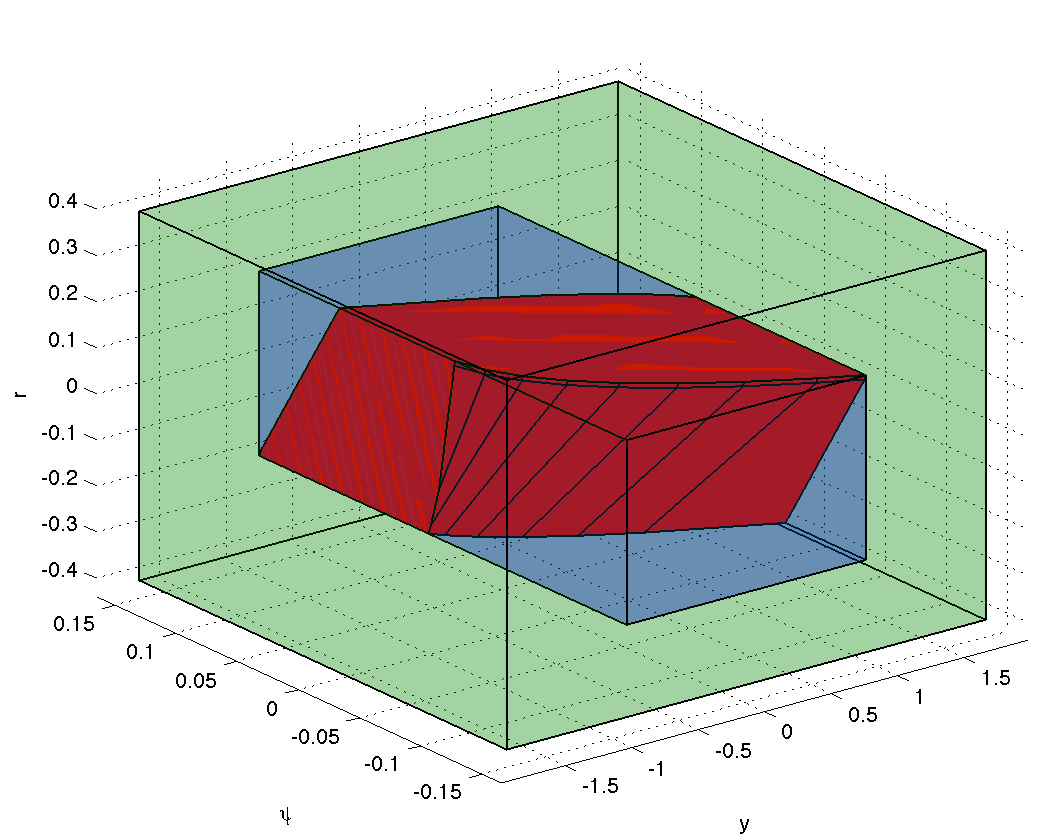
\includegraphics[width=0.4\columnwidth]{invariant}
		% This file was created by matlab2tikz v0.4.7 running on MATLAB 8.2.
% Copyright (c) 2008--2014, Nico Schlömer <nico.schloemer@gmail.com>
% All rights reserved.
% Minimal pgfplots version: 1.3
% 
\begin{tikzpicture}

\begin{axis}[%
width=\figurewidth,
height=\figureheight,
scale only axis,
xmin=0,
xmax=30,
ymin=-0.05,
ymax=0.05,
ylabel={$\psi$},
name=plot2,
axis x line*=bottom,
axis y line*=left
]
\addplot [color=blue,solid,forget plot]
  table[row sep=crcr]{0	0\\
0.1	-8.11922653108377e-11\\
0.2	-2.94274826471985e-10\\
0.3	-5.70599109401127e-10\\
0.4	-8.57046685346135e-10\\
0.5	-1.11645267556881e-09\\
0.6	-1.32502929540882e-09\\
0.7	-1.46982323270686e-09\\
0.8	-1.54639038646022e-09\\
0.9	-1.55670587213082e-09\\
1	-1.50731860379066e-09\\
1.1	-1.40775683539433e-09\\
1.2	-1.26918619845006e-09\\
1.3	-1.10331578030092e-09\\
1.4	-9.215416053197e-10\\
1.5	-7.34311210675931e-10\\
1.6	-5.50688306290393e-10\\
1.7	-3.78093033817029e-10\\
1.8	-2.22191190273808e-10\\
1.9	-8.69049355259197e-11\\
2	2.54821525094159e-11\\
2.1	1.14151446482498e-10\\
2.2	1.79530654256703e-10\\
2.3	2.230510367496e-10\\
2.4	2.4689812230643e-10\\
2.5	2.53770249125216e-10\\
2.6	2.46655935359844e-10\\
2.7	2.28637892469331e-10\\
2.8	2.02728577171907e-10\\
2.9	1.71739604727563e-10\\
3	1.38185173978418e-10\\
3.1	1.04217906866927e-10\\
3.2	7.15941827682171e-11\\
3.3	4.16651309986863e-11\\
3.4	1.53888985269601e-11\\
3.5	-6.64041181666412e-12\\
3.6	-2.41516870924157e-11\\
3.7	-3.71479214719673e-11\\
3.8	-4.58533642624988e-11\\
3.9	-5.06600209891922e-11\\
4	-5.20762313357276e-11\\
4.1	-5.06794293393911e-11\\
4.2	-4.70745870560919e-11\\
4.3	-4.18592803119233e-11\\
4.4	-3.55958134610909e-11\\
4.5	-2.87904126856009e-11\\
4.6	-2.18791508698328e-11\\
4.7	-1.52200029490366e-11\\
4.8	-9.09024632475928e-12\\
4.9	-3.68831021231078e-12\\
5	8.60868296384993e-13\\
5.1	4.49791464843484e-12\\
5.2	7.21939423898545e-12\\
5.3	9.06729166224723e-12\\
5.4	1.01182784894234e-11\\
5.5	1.04733352124429e-11\\
5.6	1.02481674685077e-11\\
5.7	9.5647336590538e-12\\
5.8	8.54408600063317e-12\\
5.9	7.30062416027075e-12\\
6	5.93777254861e-12\\
6.1	4.54502063215403e-12\\
6.2	3.19621049078042e-12\\
6.3	1.94891692214595e-12\\
6.4	8.44741617040131e-13\\
6.5	-8.96676979182726e-14\\
6.6	-8.41061618780288e-13\\
6.7	-1.40767554186092e-12\\
6.8	-1.79712026431867e-12\\
6.9	-2.02421730432732e-12\\
7	-2.10889539970274e-12\\
7.1	-2.07423936851874e-12\\
7.2	-1.94475760032252e-12\\
7.3	-1.74491116470999e-12\\
7.4	-1.4979264354358e-12\\
7.5	-1.22489509879741e-12\\
7.6	-9.44150626923299e-13\\
7.7	-6.70898863513267e-13\\
7.8	-4.17072226068556e-13\\
7.9	-1.91371873496799e-13\\
8	5.40141031669203e-16\\
8.1	1.55736803150716e-13\\
8.2	2.73646429325235e-13\\
8.3	3.55630361158349e-13\\
8.4	4.04546840681138e-13\\
8.5	4.24325022251693e-13\\
8.6	4.19568069680578e-13\\
8.7	3.95199164550798e-13\\
8.8	3.56159532808882e-13\\
8.9	3.07163309139897e-13\\
9	2.52510384703708e-13\\
9.1	1.9595529084143e-13\\
9.2	1.40627820387394e-13\\
9.3	8.89993886707929e-14\\
9.4	4.28880183054608e-14\\
9.5	3.49432082989194e-15\\
9.6	-2.85391884993143e-14\\
9.7	-5.30528190841832e-14\\
9.8	-7.02852097697565e-14\\
9.9	-8.07854979140885e-14\\
10	-8.53271235529993e-14\\
10.0137604070044	0.000614054579047492\\
10.0275208140088	0.00128969056296451\\
10.1	0.00484841859513103\\
10.1094087443329	0.00530872316761658\\
10.1188174886658	0.00576495593554063\\
10.1658612103304	0.00798504270673842\\
10.2	0.00953238122987587\\
10.3	0.01363006427895\\
10.4	0.0168826802735089\\
10.5	0.0191520106291827\\
10.6	0.0204021629209529\\
10.7	0.020668812807098\\
10.8	0.0200475444535412\\
10.9	0.0186854092399769\\
11	0.0167575524955817\\
11.1	0.0144474292229131\\
11.2	0.0119315906885171\\
11.3	0.00936874955351808\\
11.4	0.00689276486090274\\
11.5	0.00460895422618399\\
11.6	0.00258935348784601\\
11.7	0.000872722834569585\\
11.8	-0.000524728670855907\\
11.9	-0.00160350583377501\\
12	-0.00237780382095966\\
12.1	-0.00287258937294142\\
12.2	-0.00312064596669833\\
12.3	-0.00315972851254126\\
12.4	-0.00302995992190151\\
12.5	-0.00277156436998933\\
12.6	-0.00242299428789811\\
12.7	-0.00201947551423498\\
12.8	-0.00159196802777835\\
12.9	-0.00116651840079074\\
13	-0.000763964403792418\\
13.1	-0.000399941681446335\\
13.2	-8.51365656782984e-05\\
13.3	0.000174272754196068\\
13.4	0.000376043034750451\\
13.5	0.000521213240686861\\
13.6	0.000613418197219088\\
13.7	0.000658208119920864\\
13.8	0.000662406593005124\\
13.9	0.000633529826621865\\
14	0.000579283875649257\\
14.1	0.000507149327789809\\
14.2	0.000424056905803685\\
14.3	0.000336152357772449\\
14.4	0.000248644978949495\\
14.5	0.000165731119044214\\
14.6	9.0582028960938e-05\\
14.7	2.53843009753125e-05\\
14.8	-2.85791613306141e-05\\
14.9	-7.08195413263651e-05\\
15	-0.000101514274682286\\
15.1	-0.000121370816434714\\
15.2	-0.000131491114675507\\
15.3	-0.000133242393739105\\
15.4	-0.000128139630048468\\
15.5	-0.000117743253804682\\
15.6	-0.000103574173483018\\
15.7	-8.70469702464849e-05\\
15.8	-6.94210580895514e-05\\
15.9	-5.17687653894836e-05\\
16	-3.49586652091947e-05\\
16.1	-1.96520553750031e-05\\
16.2	-6.31024725714073e-06\\
16.3	4.7897590826923e-06\\
16.4	1.35335829273151e-05\\
16.5	1.99439650568632e-05\\
16.6	2.41534384984448e-05\\
16.7	2.63768545133834e-05\\
16.8	2.68851351427463e-05\\
16.9	2.5981301509983e-05\\
17	2.39795152135896e-05\\
17.1	2.11875818276354e-05\\
17.2	1.78931103648111e-05\\
17.3	1.4353306689144e-05\\
17.4	1.07882053407717e-05\\
17.5	7.37701344635041e-06\\
17.6	4.25715056328772e-06\\
17.7	1.5255160067206e-06\\
17.8	-7.58504180871018e-07\\
17.9	-2.5687702794815e-06\\
18	-3.90731154785927e-06\\
18.1	-4.79884175840963e-06\\
18.2	-5.28521369816765e-06\\
18.3	-5.42009554362819e-06\\
18.4	-5.26408707897436e-06\\
18.5	-4.88043054273421e-06\\
18.6	-4.33141221221924e-06\\
18.7	-3.67549867614996e-06\\
18.8	-2.96520740893803e-06\\
18.9	-2.24567541829736e-06\\
19	-1.55386252021772e-06\\
19.1	-9.18306884296458e-07\\
19.2	-3.59339224911901e-07\\
19.3	1.10342520371231e-07\\
19.4	4.84835049999351e-07\\
19.5	7.64019457494767e-07\\
19.6	9.52461203905629e-07\\
19.7	1.05829127235434e-06\\
19.8	1.09212682621428e-06\\
19.9	1.06607661058417e-06\\
19.9605807921388	1.02672971263974e-06\\
19.9893482375409	1.00295717234103e-06\\
20	-6.74949728054996e-05\\
20.0100988555802	-0.00101399150051312\\
20.0264373103001	-0.00261826984190363\\
20.1	-0.00983939558936009\\
20.2	-0.0192719072640704\\
20.3	-0.0275059673728831\\
20.4	-0.0340085394562876\\
20.5	-0.0385113162665394\\
20.6	-0.0409324133727168\\
20.7	-0.0413403921563173\\
20.8	-0.0399569880755265\\
20.9	-0.0370972929098225\\
21	-0.0331254805447789\\
21.1	-0.0284166011413822\\
21.2	-0.0233272723903758\\
21.3	-0.0181749791343795\\
21.4	-0.0132252703628319\\
21.5	-0.00868572216082228\\
21.6	-0.00470226024621395\\
21.7	-0.00136023147536542\\
21.8	0.00131226176933267\\
21.9	0.00333428972721868\\
22	0.004748870330059\\
22.1	0.0056164173463112\\
22.2	0.00600943157908607\\
22.3	0.00600734657530052\\
22.4	0.00569188130898003\\
22.5	0.00514303829922637\\
22.6	0.00443585256480859\\
22.7	0.00363792456179008\\
22.8	0.0028077266100698\\
22.9	0.00199364014010824\\
23	0.00123363370392003\\
23.1	0.000555485640447223\\
23.2	-2.25577867284188e-05\\
23.3	-0.000490798946614331\\
23.4	-0.000846888111874368\\
23.5	-0.00109450391757043\\
23.6	-0.0012420012115514\\
23.7	-0.00130109731725597\\
23.8	-0.00128564792826097\\
23.9	-0.00121055200895605\\
24	-0.00109081423037325\\
24.1	-0.000940781160305623\\
24.2	-0.000773556371320787\\
24.3	-0.00060058971134406\\
24.4	-0.000431428085179353\\
24.5	-0.000273609108256015\\
24.6	-0.000132674853282432\\
24.7	-1.22816131058815e-05\\
24.8	8.56184398777887e-05\\
24.9	0.000160546677292676\\
25	0.000213239376186438\\
25.1	0.000245379238140286\\
25.2	0.000259331956161445\\
25.3	0.000257899642901094\\
25.4	0.000244100308459425\\
25.5	0.000220979018302501\\
25.6	0.000191453850237237\\
25.7	0.000158197515905028\\
25.8	0.000123553609828142\\
25.9	8.94849583198706e-05\\
26	5.75504577925253e-05\\
26.1	2.89060925715187e-05\\
26.2	4.32550223935401e-06\\
26.3	-1.5764720247289e-05\\
26.4	-3.12395868783966e-05\\
26.5	-4.22241254479661e-05\\
26.6	-4.90394115179308e-05\\
26.7	-5.21493242750464e-05\\
26.8	-5.21104915086262e-05\\
26.9	-4.95272716108671e-05\\
27	-4.50130177500795e-05\\
27.1	-3.91583071415736e-05\\
27.2	-3.25063671634784e-05\\
27.3	-2.55355245792479e-05\\
27.4	-1.86481937590884e-05\\
27.5	-1.21656918754936e-05\\
27.6	-6.32801967319582e-06\\
27.7	-1.29766792380124e-06\\
27.8	2.83350765937696e-06\\
27.9	6.03526733097167e-06\\
28	8.32867638394659e-06\\
28.1	9.77525477731482e-06\\
28.2	1.04662220597865e-05\\
28.3	1.05123461177986e-05\\
28.4	1.00347773372869e-05\\
28.5	9.15712845637148e-06\\
28.6	7.99894956122152e-06\\
28.7	6.67065075458052e-06\\
28.8	5.26984408623537e-06\\
28.9	3.87901227761926e-06\\
29	2.56436450143962e-06\\
29.1	1.3757080925907e-06\\
29.2	3.47148064767023e-07\\
29.3	-5.01578231279225e-07\\
29.4	-1.16331820898364e-06\\
29.5	-1.64144599600194e-06\\
29.6	-1.94768267726972e-06\\
29.7	-2.09992487462657e-06\\
29.8	-2.12018641441149e-06\\
29.9	-2.03273225131636e-06\\
29.9695899823905	-1.92193131798056e-06\\
30	0.000193666027198354\\
};
\end{axis}

\begin{axis}[%
width=\figurewidth,
height=\figureheight,
scale only axis,
xmin=0,
xmax=30,
ymin=-1,
ymax=1,
ylabel={$y$},
at=(plot2.above north west),
anchor=below south west
]
\addplot [color=blue,solid,forget plot]
  table[row sep=crcr]{0	0\\
0.1	-8.11922653108378e-11\\
0.2	-6.22345811225611e-10\\
0.3	-1.91264499689916e-09\\
0.4	-4.05789244489903e-09\\
0.5	-7.02909455764372e-09\\
0.6	-1.07064855297974e-08\\
0.7	-1.49157931201043e-08\\
0.8	-1.94571964277945e-08\\
0.9	-2.41276582308046e-08\\
1	-2.87373521778653e-08\\
1.1	-3.31209291850559e-08\\
1.2	-3.7144379663253e-08\\
1.3	-4.07082439563006e-08\\
1.4	-4.37479006583683e-08\\
1.5	-4.62316218523658e-08\\
1.6	-4.81570280424602e-08\\
1.7	-4.95465069811747e-08\\
1.8	-5.04420835780727e-08\\
1.9	-5.09001465907383e-08\\
2	-5.09863555980291e-08\\
2.1	-5.07709721679858e-08\\
2.2	-5.03247849151831e-08\\
2.3	-4.9715731411967e-08\\
2.4	-4.90062621330795e-08\\
2.5	-4.82514436042183e-08\\
2.6	-4.74977599518466e-08\\
2.7	-4.67825438847491e-08\\
2.8	-4.61339491514712e-08\\
2.9	-4.55713657872049e-08\\
3	-4.51061758589867e-08\\
3.1	-4.47427496960268e-08\\
3.2	-4.4479589471788e-08\\
3.3	-4.43105372359172e-08\\
3.4	-4.4225976909999e-08\\
3.5	-4.42139733162574e-08\\
3.6	-4.42613051070704e-08\\
3.7	-4.43543617720641e-08\\
3.8	-4.44798871521294e-08\\
3.9	-4.46255626821258e-08\\
4	-4.47804326618321e-08\\
4.1	-4.49351810982285e-08\\
4.2	-4.50822750639139e-08\\
4.3	-4.52159931627253e-08\\
4.4	-4.53323597392513e-08\\
4.5	-4.54290061187781e-08\\
4.6	-4.55049796523066e-08\\
4.7	-4.55605199138197e-08\\
4.8	-4.55968192978328e-08\\
4.9	-4.56157827259647e-08\\
5	-4.56197983987336e-08\\
5.1	-4.56115287036417e-08\\
5.2	-4.55937276607014e-08\\
5.3	-4.55690887668236e-08\\
5.4	-4.55401248740666e-08\\
5.5	-4.55090798563096e-08\\
5.6	-4.54778703103373e-08\\
5.7	-4.54480544029221e-08\\
5.8	-4.54208241995072e-08\\
5.9	-4.53970173617802e-08\\
6	-4.5377143940118e-08\\
6.1	-4.53614240654039e-08\\
6.2	-4.5349832613442e-08\\
6.3	-4.53421473248804e-08\\
6.4	-4.53379973668285e-08\\
6.5	-4.53369098766911e-08\\
6.6	-4.53383525977034e-08\\
6.7	-4.5341771268158e-08\\
6.8	-4.53466209386741e-08\\
6.9	-4.53523908466393e-08\\
7	-4.53586228629378e-08\\
7.1	-4.53649238376667e-08\\
7.2	-4.53709724073243e-08\\
7.3	-4.53765209894159e-08\\
7.4	-4.53813937870204e-08\\
7.5	-4.53854816636962e-08\\
7.6	-4.53887347377288e-08\\
7.7	-4.53911534939206e-08\\
7.8	-4.53927791311287e-08\\
7.9	-4.53936837637557e-08\\
8	-4.5393960984349e-08\\
8.1	-4.53937171798874e-08\\
8.2	-4.5393063882387e-08\\
8.3	-4.53921113302243e-08\\
8.4	-4.53909633235886e-08\\
8.5	-4.53897133783923e-08\\
8.6	-4.53884421184727e-08\\
8.7	-4.53872157968882e-08\\
8.8	-4.53860858027661e-08\\
8.9	-4.53850889894546e-08\\
9	-4.53842486508936e-08\\
9.1	-4.53835759745144e-08\\
9.2	-4.53830718085259e-08\\
9.3	-4.53827285970246e-08\\
9.4	-4.53825323562007e-08\\
9.5	-4.53824645871586e-08\\
9.6	-4.53825040439052e-08\\
9.7	-4.53826282976775e-08\\
9.8	-4.53828150600751e-08\\
9.9	-4.5383043246334e-08\\
10	-4.53832937764988e-08\\
10.0137604070044	0.000113988452741948\\
10.0275208140088	0.0005069330725436\\
10.1	0.00718021040209756\\
10.1094087443329	0.00861379492966521\\
10.1188174886658	0.0101767319386806\\
10.1658612103304	0.0198914706264442\\
10.2	0.0288664005739314\\
10.3	0.0638018952095956\\
10.4	0.109809562719548\\
10.5	0.164117492751253\\
10.6	0.223701844051563\\
10.7	0.285543864442493\\
10.8	0.346821053516602\\
10.9	0.405080958398762\\
11	0.458359854276093\\
11.1	0.505236170299817\\
11.2	0.544831512132066\\
11.3	0.576772502048684\\
11.4	0.601125855532693\\
11.5	0.618317532039055\\
11.6	0.629041723865359\\
11.7	0.634155643979458\\
11.8	0.634597023939803\\
11.9	0.631326365001092\\
12	0.62528139817381\\
12.1	0.617340367970257\\
12.2	0.608294162107008\\
12.3	0.59882717817003\\
12.4	0.589506391205977\\
12.5	0.580777744440386\\
12.6	0.572968758767489\\
12.7	0.566296135831338\\
12.8	0.560877098177314\\
12.9	0.556743251035294\\
13	0.553855846789594\\
13.1	0.552121468893313\\
13.2	0.551407312079936\\
13.3	0.551555407195845\\
13.4	0.55239531086036\\
13.5	0.553754943814516\\
13.6	0.555469410478052\\
13.7	0.55738775880943\\
13.8	0.55937775018276\\
13.9	0.561328790156782\\
14	0.563153230911004\\
14.1	0.564786295111131\\
14.2	0.566184890153367\\
14.3	0.567325584207491\\
14.4	0.568202004291332\\
14.5	0.568821894899983\\
14.6	0.569204046538715\\
14.7	0.569375269711571\\
14.8	0.569367554026461\\
14.9	0.569215516093975\\
15	0.56895420569878\\
15.1	0.568617311025397\\
15.2	0.568235772822881\\
15.3	0.567836797241628\\
15.4	0.567443239822103\\
15.5	0.567073319879205\\
15.6	0.566740616127064\\
15.7	0.566454290020731\\
15.8	0.566219482379083\\
15.9	0.566037830779593\\
16	0.565908059343153\\
16.1	0.565826598232834\\
16.2	0.565788196893488\\
16.3	0.565786502240563\\
16.4	0.565814580223768\\
16.5	0.565865366084228\\
16.6	0.565932034917361\\
16.7	0.56600828965451\\
16.8	0.566088568166993\\
16.9	0.566168174825946\\
17	0.56624334452641\\
17.1	0.566311248956128\\
17.2	0.566369955844457\\
17.3	0.56641835217409\\
17.4	0.566456042001205\\
17.5	0.56648322873631\\
17.6	0.566500590614509\\
17.7	0.566509156748277\\
17.8	0.566510189713884\\
17.9	0.566505079165322\\
18	0.566495249571062\\
18.1	0.56648208388643\\
18.2	0.566466863848406\\
18.3	0.566450726635279\\
18.4	0.566434636882449\\
18.5	0.566419372487375\\
18.6	0.566405522261817\\
18.7	0.566393493281285\\
18.8	0.566383525718351\\
18.9	0.566375713003575\\
19	0.566370025309434\\
19.1	0.566366334573353\\
19.2	0.566364439541696\\
19.3	0.566364089605778\\
19.4	0.566365006494991\\
19.5	0.56636690317568\\
19.6	0.566369499565599\\
19.7	0.566372534904123\\
19.8	0.566375776812514\\
19.9	0.566379027233886\\
19.9605807921388	0.566380931196237\\
19.9893482375409	0.566381807265479\\
20	0.566382126236082\\
20.0100988555802	0.566225144304234\\
20.0264373103001	0.565334954583245\\
20.1	0.551588056163345\\
20.2	0.507689355078309\\
20.3	0.437127397315184\\
20.4	0.344369915836634\\
20.5	0.235070466823728\\
20.6	0.115383622319823\\
20.7	-0.00850310112939186\\
20.8	-0.130854825505024\\
20.9	-0.246753431860216\\
21	-0.352310167653342\\
21.1	-0.444753362138088\\
21.2	-0.522414873788062\\
21.3	-0.584641685010991\\
21.4	-0.631657442445099\\
21.5	-0.664396137533923\\
21.6	-0.684323320370016\\
21.7	-0.693248921630284\\
21.8	-0.693154669729446\\
21.9	-0.686027356266407\\
22	-0.673758749406503\\
22.1	-0.65808414481232\\
22.2	-0.640538131879383\\
22.3	-0.622426175687266\\
22.4	-0.604810937232511\\
22.5	-0.588511600941238\\
22.6	-0.574114097718101\\
22.7	-0.561989902311225\\
22.8	-0.552321069467567\\
22.9	-0.54512923171826\\
23	-0.540306502414787\\
23.1	-0.537646500612299\\
23.2	-0.536874027267137\\
23.3	-0.537672251437246\\
23.4	-0.539706594112297\\
23.5	-0.542644809150187\\
23.6	-0.546173036442427\\
23.7	-0.550007842030949\\
23.8	-0.553904440636819\\
23.9	-0.557661430918173\\
24	-0.56112247649106\\
24.1	-0.564175432511554\\
24.2	-0.566749449450244\\
24.3	-0.56881058595625\\
24.4	-0.57035643586435\\
24.5	-0.571410227355509\\
24.6	-0.572014789180624\\
24.7	-0.572226708245357\\
24.8	-0.572110930261419\\
24.9	-0.571735984228069\\
25	-0.571169945576751\\
25.1	-0.570477194145341\\
25.2	-0.569715973137887\\
25.3	-0.568936715821924\\
25.4	-0.568181074545866\\
25.5	-0.567481564829261\\
25.6	-0.566861724211731\\
25.7	-0.566336679647385\\
25.8	-0.565914017590953\\
25.9	-0.565594856372638\\
26	-0.565375029765342\\
26.1	-0.565246302619204\\
26.2	-0.565197552948924\\
26.3	-0.565215868967892\\
26.4	-0.565287524021536\\
26.5	-0.565398804962045\\
26.6	-0.565536681346025\\
26.7	-0.565689313130931\\
26.8	-0.565846402900772\\
26.9	-0.565999405105096\\
27	-0.566141609449314\\
27.1	-0.566268118420896\\
27.2	-0.5663757403063\\
27.3	-0.566462819114791\\
27.4	-0.566529021817705\\
27.5	-0.566575101497198\\
27.6	-0.56660265261971\\
27.7	-0.566613871931067\\
27.8	-0.566611335610728\\
27.9	-0.566597800489512\\
28	-0.566576034462092\\
28.1	-0.566548678813032\\
28.2	-0.566518143091405\\
28.3	-0.566486531453233\\
28.4	-0.566455598056668\\
28.5	-0.566426728134206\\
28.6	-0.566400940754884\\
28.7	-0.566378908990236\\
28.8	-0.566360993165853\\
28.9	-0.566347283065936\\
29	-0.566337645310651\\
29.1	-0.566331772596181\\
29.2	-0.566329232029567\\
29.3	-0.56632951036443\\
29.4	-0.566332054515255\\
29.5	-0.566336306269576\\
29.6	-0.566341730608368\\
29.7	-0.566347837470818\\
29.8	-0.566354197152053\\
29.9	-0.566360449798163\\
29.9695899823905	-0.566364583627999\\
30	-0.566366310671168\\
};
\end{axis}

\begin{axis}[%
width=\figurewidth,
height=\figureheight,
scale only axis,
xmin=0,
xmax=30,
ymin=-0.1,
ymax=0.3,
ylabel={$r$},
at=(plot2.below south west),
anchor=above north west,
axis x line*=bottom,
axis y line*=left
]
\addplot [color=red,solid,forget plot]
  table[row sep=crcr]{0	0\\
0.1	0\\
0.2	0\\
0.3	0\\
0.4	0\\
0.5	0\\
0.6	0\\
0.7	0\\
0.8	0\\
0.9	0\\
1	0\\
1.1	0\\
1.2	0\\
1.3	0\\
1.4	0\\
1.5	0\\
1.6	0\\
1.7	0\\
1.8	0\\
1.9	0\\
2	0\\
2.1	0\\
2.2	0\\
2.3	0\\
2.4	0\\
2.5	0\\
2.6	0\\
2.7	0\\
2.8	0\\
2.9	0\\
3	0\\
3.1	0\\
3.2	0\\
3.3	0\\
3.4	0\\
3.5	0\\
3.6	0\\
3.7	0\\
3.8	0\\
3.9	0\\
4	0\\
4.1	0\\
4.2	0\\
4.3	0\\
4.4	0\\
4.5	0\\
4.6	0\\
4.7	0\\
4.8	0\\
4.9	0\\
5	0\\
5.1	0\\
5.2	0\\
5.3	0\\
5.4	0\\
5.5	0\\
5.6	0\\
5.7	0\\
5.8	0\\
5.9	0\\
6	0\\
6.1	0\\
6.2	0\\
6.3	0\\
6.4	0\\
6.5	0\\
6.6	0\\
6.7	0\\
6.8	0\\
6.9	0\\
7	0\\
7.1	0\\
7.2	0\\
7.3	0\\
7.4	0\\
7.5	0\\
7.6	0\\
7.7	0\\
7.8	0\\
7.9	0\\
8	0\\
8.1	0\\
8.2	0\\
8.3	0\\
8.4	0\\
8.5	0\\
8.6	0\\
8.7	0\\
8.8	0\\
8.9	0\\
9	0\\
9.1	0\\
9.2	0\\
9.3	0\\
9.4	0\\
9.5	0\\
9.6	0\\
9.7	0\\
9.8	0\\
9.9	0\\
10	0\\
10.0137604070044	0.0491\\
10.0275208140088	0.0491\\
10.1	0.0491\\
10.1094087443329	0.0491\\
10.1188174886658	0.0491\\
10.1658612103304	0.0491\\
10.2	0.0491\\
10.3	0.0491\\
10.4	0.0491\\
10.5	0.0491\\
10.6	0.0491\\
10.7	0.0491\\
10.8	0.0491\\
10.9	0.0491\\
11	0.0491\\
11.1	0.0491\\
11.2	0.0491\\
11.3	0.0491\\
11.4	0.0491\\
11.5	0.0491\\
11.6	0.0491\\
11.7	0.0491\\
11.8	0.0491\\
11.9	0.0491\\
12	0.0491\\
12.1	0.0491\\
12.2	0.0491\\
12.3	0.0491\\
12.4	0.0491\\
12.5	0.0491\\
12.6	0.0491\\
12.7	0.0491\\
12.8	0.0491\\
12.9	0.0491\\
13	0.0491\\
13.1	0.0491\\
13.2	0.0491\\
13.3	0.0491\\
13.4	0.0491\\
13.5	0.0491\\
13.6	0.0491\\
13.7	0.0491\\
13.8	0.0491\\
13.9	0.0491\\
14	0.0491\\
14.1	0.0491\\
14.2	0.0491\\
14.3	0.0491\\
14.4	0.0491\\
14.5	0.0491\\
14.6	0.0491\\
14.7	0.0491\\
14.8	0.0491\\
14.9	0.0491\\
15	0.0491\\
15.1	0.0491\\
15.2	0.0491\\
15.3	0.0491\\
15.4	0.0491\\
15.5	0.0491\\
15.6	0.0491\\
15.7	0.0491\\
15.8	0.0491\\
15.9	0.0491\\
16	0.0491\\
16.1	0.0491\\
16.2	0.0491\\
16.3	0.0491\\
16.4	0.0491\\
16.5	0.0491\\
16.6	0.0491\\
16.7	0.0491\\
16.8	0.0491\\
16.9	0.0491\\
17	0.0491\\
17.1	0.0491\\
17.2	0.0491\\
17.3	0.0491\\
17.4	0.0491\\
17.5	0.0491\\
17.6	0.0491\\
17.7	0.0491\\
17.8	0.0491\\
17.9	0.0491\\
18	0.0491\\
18.1	0.0491\\
18.2	0.0491\\
18.3	0.0491\\
18.4	0.0491\\
18.5	0.0491\\
18.6	0.0491\\
18.7	0.0491\\
18.8	0.0491\\
18.9	0.0491\\
19	0.0491\\
19.1	0.0491\\
19.2	0.0491\\
19.3	0.0491\\
19.4	0.0491\\
19.5	0.0491\\
19.6	0.0491\\
19.7	0.0491\\
19.8	0.0491\\
19.9	0.0491\\
19.9605807921388	0.0491\\
19.9893482375409	0.0491\\
20	0\\
20.0100988555802	-0.0491\\
20.0264373103001	-0.0491\\
20.1	-0.0491\\
20.2	-0.0491\\
20.3	-0.0491\\
20.4	-0.0491\\
20.5	-0.0491\\
20.6	-0.0491\\
20.7	-0.0491\\
20.8	-0.0491\\
20.9	-0.0491\\
21	-0.0491\\
21.1	-0.0491\\
21.2	-0.0491\\
21.3	-0.0491\\
21.4	-0.0491\\
21.5	-0.0491\\
21.6	-0.0491\\
21.7	-0.0491\\
21.8	-0.0491\\
21.9	-0.0491\\
22	-0.0491\\
22.1	-0.0491\\
22.2	-0.0491\\
22.3	-0.0491\\
22.4	-0.0491\\
22.5	-0.0491\\
22.6	-0.0491\\
22.7	-0.0491\\
22.8	-0.0491\\
22.9	-0.0491\\
23	-0.0491\\
23.1	-0.0491\\
23.2	-0.0491\\
23.3	-0.0491\\
23.4	-0.0491\\
23.5	-0.0491\\
23.6	-0.0491\\
23.7	-0.0491\\
23.8	-0.0491\\
23.9	-0.0491\\
24	-0.0491\\
24.1	-0.0491\\
24.2	-0.0491\\
24.3	-0.0491\\
24.4	-0.0491\\
24.5	-0.0491\\
24.6	-0.0491\\
24.7	-0.0491\\
24.8	-0.0491\\
24.9	-0.0491\\
25	-0.0491\\
25.1	-0.0491\\
25.2	-0.0491\\
25.3	-0.0491\\
25.4	-0.0491\\
25.5	-0.0491\\
25.6	-0.0491\\
25.7	-0.0491\\
25.8	-0.0491\\
25.9	-0.0491\\
26	-0.0491\\
26.1	-0.0491\\
26.2	-0.0491\\
26.3	-0.0491\\
26.4	-0.0491\\
26.5	-0.0491\\
26.6	-0.0491\\
26.7	-0.0491\\
26.8	-0.0491\\
26.9	-0.0491\\
27	-0.0491\\
27.1	-0.0491\\
27.2	-0.0491\\
27.3	-0.0491\\
27.4	-0.0491\\
27.5	-0.0491\\
27.6	-0.0491\\
27.7	-0.0491\\
27.8	-0.0491\\
27.9	-0.0491\\
28	-0.0491\\
28.1	-0.0491\\
28.2	-0.0491\\
28.3	-0.0491\\
28.4	-0.0491\\
28.5	-0.0491\\
28.6	-0.0491\\
28.7	-0.0491\\
28.8	-0.0491\\
28.9	-0.0491\\
29	-0.0491\\
29.1	-0.0491\\
29.2	-0.0491\\
29.3	-0.0491\\
29.4	-0.0491\\
29.5	-0.0491\\
29.6	-0.0491\\
29.7	-0.0491\\
29.8	-0.0491\\
29.9	-0.0491\\
29.9695899823905	-0.0491\\
30	0\\
};
\addplot [color=blue,solid,forget plot]
  table[row sep=crcr]{0	0\\
0.1	-1.62384530621676e-09\\
0.2	-2.56982513885346e-09\\
0.3	-2.9019129764928e-09\\
0.4	-2.78777893891346e-09\\
0.5	-2.37425311034735e-09\\
0.6	-1.78196843166073e-09\\
0.7	-1.10717085431314e-09\\
0.8	-4.2400930397745e-10\\
0.9	2.1306091209435e-10\\
1	7.66791843802708e-10\\
1.1	1.21461380305122e-09\\
1.2	1.54611979988266e-09\\
1.3	1.76062603629072e-09\\
1.4	1.86486883311251e-09\\
1.5	1.87089053142448e-09\\
1.6	1.7941555655891e-09\\
1.7	1.65192486674047e-09\\
1.8	1.46190340497729e-09\\
1.9	1.24116306611726e-09\\
2	1.00533191335327e-09\\
2.1	7.68031671638409e-10\\
2.2	5.4053820739258e-10\\
2.3	3.31634933395339e-10\\
2.4	1.47626322198127e-10\\
2.5	-7.52211844916736e-12\\
2.6	-1.31950253290517e-10\\
2.7	-2.25606828081685e-10\\
2.8	-2.89917677867181e-10\\
2.9	-3.27442428719796e-10\\
3	-3.41539314335309e-10\\
3.1	-3.36053430746415e-10\\
3.2	-3.15039565694807e-10\\
3.3	-2.82526832468088e-10\\
3.4	-2.42328843792384e-10\\
3.5	-1.97900171487145e-10\\
3.6	-1.5223739111503e-10\\
3.7	-1.07821124509785e-10\\
3.8	-6.65941535546279e-11\\
3.9	-2.99698350060208e-11\\
4	1.13534129054239e-12\\
4.1	2.625122849028e-11\\
4.2	4.52914101919645e-11\\
4.3	5.84838549218295e-11\\
4.4	6.62995006535585e-11\\
4.5	6.93826462158838e-11\\
4.6	6.84861994741817e-11\\
4.7	6.44140165506907e-11\\
4.8	5.79717874777038e-11\\
4.9	4.99272362643543e-11\\
5	4.09797961955214e-11\\
5.1	3.17394300020004e-11\\
5.2	2.27138814253823e-11\\
5.3	1.4303368027481e-11\\
5.4	6.80155148247289e-12\\
5.5	4.01536091264669e-13\\
5.6	-4.79435838212933e-12\\
5.7	-8.76225065368174e-12\\
5.8	-1.15428742854209e-11\\
5.9	-1.32272359268889e-11\\
6	-1.39425554994846e-11\\
6.1	-1.38391220008252e-11\\
6.2	-1.30785342036062e-11\\
6.3	-1.18236359222703e-11\\
6.4	-1.02303134362168e-11\\
6.5	-8.44120201255207e-12\\
6.6	-6.58124323053848e-12\\
6.7	-4.75495700968715e-12\\
6.8	-3.04523384239983e-12\\
6.9	-1.51341554309328e-12\\
7	-2.00415213892061e-13\\
7.1	8.71378783466446e-13\\
7.2	1.6956560386774e-12\\
7.3	2.27941884316326e-12\\
7.4	2.64009477855571e-12\\
7.5	2.80269111708154e-12\\
7.6	2.79712287316286e-12\\
7.7	2.65581100158589e-12\\
7.8	2.41161773576783e-12\\
7.9	2.09615495262284e-12\\
8	1.73847694177762e-12\\
8.1	1.36414834456637e-12\\
8.2	9.94660846332281e-13\\
8.3	6.47161013638343e-13\\
8.4	3.344416533772e-13\\
8.5	6.51488292840089e-14\\
8.6	-1.55848313190869e-13\\
8.7	-3.26973536359827e-13\\
8.8	-4.4939133007026e-13\\
8.9	-5.26425858525353e-13\\
9	-5.62985443829235e-13\\
9.1	-5.65019779508147e-13\\
9.2	-5.39029712025691e-13\\
9.3	-4.9164392815298e-13\\
9.4	-4.2927045850378e-13\\
9.5	-3.57825412339134e-13\\
9.6	-2.82537408117159e-13\\
9.7	-2.0782361378229e-13\\
9.8	-1.37228368590926e-13\\
9.9	-7.34172146084666e-14\\
10	-1.8214437033076e-14\\
10.0137604070044	-1.19478980935457e-14\\
10.0275208140088	-5.8036709334889e-15\\
10.1	2.65593676715862e-14\\
10.1094087443329	-0.000393323105652787\\
10.1188174886658	-0.00082609122193077\\
10.1658612103304	-0.00298993180332068\\
10.2	-0.00456019231572906\\
10.3	-0.0119677425535038\\
10.4	-0.0213497041539368\\
10.5	-0.0315263606220314\\
10.6	-0.0416599937327086\\
10.7	-0.0511428026618412\\
10.8	-0.0593623113982453\\
10.9	-0.0659264403291893\\
11	-0.0706628369933811\\
11.1	-0.0735733508576698\\
11.2	-0.0747902483171021\\
11.3	-0.0745342208930131\\
11.4	-0.0730784256800208\\
11.5	-0.070717777886746\\
11.6	-0.0678293294182144\\
11.7	-0.0646818054803717\\
11.8	-0.0614621441945055\\
11.9	-0.0583218700212347\\
12	-0.0553834871813748\\
12.1	-0.052739836189547\\
12.2	-0.0504544563081405\\
12.3	-0.0485634159927314\\
12.4	-0.047078287129696\\
12.5	-0.0459898683991183\\
12.6	-0.0452723047371501\\
12.7	-0.0448873043047814\\
12.8	-0.0447882116197382\\
12.9	-0.0449237525087443\\
13	-0.0452413207741734\\
13.1	-0.0456897260148116\\
13.2	-0.0462213655273006\\
13.3	-0.0467938197988688\\
13.4	-0.0473709004112481\\
13.5	-0.0479231973868444\\
13.6	-0.0484282122472045\\
13.7	-0.0488701099036248\\
13.8	-0.0492392096042514\\
13.9	-0.0495312730505288\\
14	-0.0497466640424109\\
14.1	-0.0498894453327554\\
14.2	-0.0499664684964771\\
14.3	-0.049986502367031\\
14.4	-0.0499594350738026\\
14.5	-0.0498955744707279\\
14.6	-0.0498050622324983\\
14.7	-0.0496974084421774\\
14.8	-0.049581146317633\\
14.9	-0.0494636046107615\\
15	-0.0493507675526612\\
15.1	-0.0492472500187035\\
15.2	-0.0491563304218345\\
15.3	-0.0490800449844573\\
15.4	-0.0490193254198734\\
15.5	-0.0489741643904854\\
15.6	-0.0489437952952349\\
15.7	-0.0489268748444177\\
15.8	-0.0489216589538643\\
15.9	-0.0489261646286284\\
16	-0.0489383125938034\\
16.1	-0.0489560473746637\\
16.2	-0.0489774332622805\\
16.3	-0.0490007260795864\\
16.4	-0.0490244218630396\\
16.5	-0.049047284491161\\
16.6	-0.0490683549328025\\
16.7	-0.0490869451761602\\
16.8	-0.0491026200637576\\
16.9	-0.0491151702336631\\
17	-0.0491245791904737\\
17.1	-0.0491309872387465\\
17.2	-0.0491346546426426\\
17.3	-0.0491359259615299\\
17.4	-0.049135197081051\\
17.5	-0.0491328860368463\\
17.6	-0.0491294083328715\\
17.7	-0.0491251571022272\\
17.8	-0.0491204881550568\\
17.9	-0.0491157097105217\\
18	-0.0491110764195715\\
18.1	-0.049106787150548\\
18.2	-0.0491029859265545\\
18.3	-0.0490997653661891\\
18.4	-0.0490971719807601\\
18.5	-0.0490952127139704\\
18.6	-0.0490938621666722\\
18.7	-0.0490930700223493\\
18.8	-0.0490927682717612\\
18.9	-0.0490928779217792\\
19	-0.0490933149588859\\
19.1	-0.0490939954181478\\
19.2	-0.0490948394807429\\
19.3	-0.0490957745853474\\
19.4	-0.0490967375897254\\
19.5	-0.0490976760583746\\
19.6	-0.0490985487803272\\
19.7	-0.0490993256389529\\
19.8	-0.0490999869640176\\
19.9	-0.0491005224966669\\
19.9605807921388	-0.0491007694211242\\
19.9893482375409	-0.0491008833179332\\
20	-0.0491009254906649\\
20.0100988555802	-0.0490953238915918\\
20.0264373103001	-0.0490853459928587\\
20.1	-0.0490404212382876\\
20.2	-0.0405660738373393\\
20.3	-0.025320701304647\\
20.4	-0.00620190071981568\\
20.5	0.0144690456460339\\
20.6	0.0353141774153078\\
20.7	0.054565934935014\\
20.8	0.0710396206207114\\
20.9	0.0840314246858735\\
21	0.0932597774414358\\
21.1	0.0987805985121892\\
21.2	0.100898530381745\\
21.3	0.100084089997604\\
21.4	0.0968987122474094\\
21.5	0.0919351185662022\\
21.6	0.085836000243047\\
21.7	0.0791561785044741\\
21.8	0.072501012568649\\
21.9	0.0661714672330136\\
22	0.0603698918934955\\
22.1	0.0552438015152278\\
22.2	0.0508873769688907\\
22.3	0.0473455015689265\\
22.4	0.0446195389367532\\
22.5	0.0426744567777358\\
22.6	0.0414466563370838\\
22.7	0.0408517533369504\\
22.8	0.0407922696812227\\
22.9	0.0411644822872263\\
23	0.0418643935924598\\
23.1	0.0427926347791445\\
23.2	0.0438582708412469\\
23.3	0.0449815010925071\\
23.4	0.0460953099317408\\
23.5	0.0471462055781819\\
23.6	0.0480941416927738\\
23.7	0.048911849515529\\
23.8	0.049583725417649\\
23.9	0.0501043718134783\\
24	0.050476917307969\\
24.1	0.0507112318989239\\
24.2	0.0508221429746816\\
24.3	0.0508277443580303\\
24.4	0.0507478626562663\\
24.5	0.0506027386983928\\
24.6	0.0504119459060242\\
24.7	0.0501935520814613\\
24.8	0.0499635190858796\\
24.9	0.0497353231504941\\
25	0.0495197710004604\\
25.1	0.0493249843676893\\
25.2	0.0491565126503963\\
25.3	0.0490175560916486\\
25.4	0.0489092597474727\\
25.5	0.0488310507491811\\
25.6	0.0487809948524407\\
25.7	0.0487561512920619\\
25.8	0.0487529089648239\\
25.9	0.0487672911088803\\
26	0.0487952196395914\\
26.1	0.0488327339618272\\
26.2	0.0488761630737491\\
26.3	0.0489222477653778\\
26.4	0.0489682222601679\\
26.5	0.0490118554395746\\
26.6	0.0490514578237774\\
26.7	0.0490858606901638\\
26.8	0.0491143737593799\\
26.9	0.0491367272963834\\
27	0.0491530049468748\\
27.1	0.0491635720123209\\
27.2	0.0491690036461126\\
27.3	0.0491700165091958\\
27.4	0.0491674065724802\\
27.5	0.0491619949389031\\
27.6	0.0491545828058234\\
27.7	0.0491459160251865\\
27.8	0.0491366591603837\\
27.9	0.0491273784923623\\
28	0.0491185330937179\\
28.1	0.0491104728629773\\
28.2	0.0491034422825328\\
28.3	0.0490975886202317\\
28.4	0.0490929733221893\\
28.5	0.0490895854279965\\
28.6	0.0490873559642828\\
28.7	0.0490861724245816\\
28.8	0.0490858926099689\\
28.9	0.0490863572751023\\
29	0.0490874011890439\\
29.1	0.0490888623726018\\
29.2	0.0490905894087846\\
29.3	0.0490924468370889\\
29.4	0.0490943187341085\\
29.5	0.049096110652156\\
29.6	0.0490977501351434\\
29.7	0.0490991860586958\\
29.8	0.0491003870518034\\
29.9	0.0491013392530631\\
29.9695899823905	0.0491018294349302\\
30	0.0491020367757445\\
};
\end{axis}
\end{tikzpicture}%
	\end{center}
	\caption{Car states in simulation. Yellow line is $r_{road}$.}
	\label{fig:invariant}
\end{figure}
\setlength\figurewidth{0.5\columnwidth} 
\setlength\figureheight{0.2 \columnwidth} 

\begin{figure}[ht]
	\begin{center}
		% 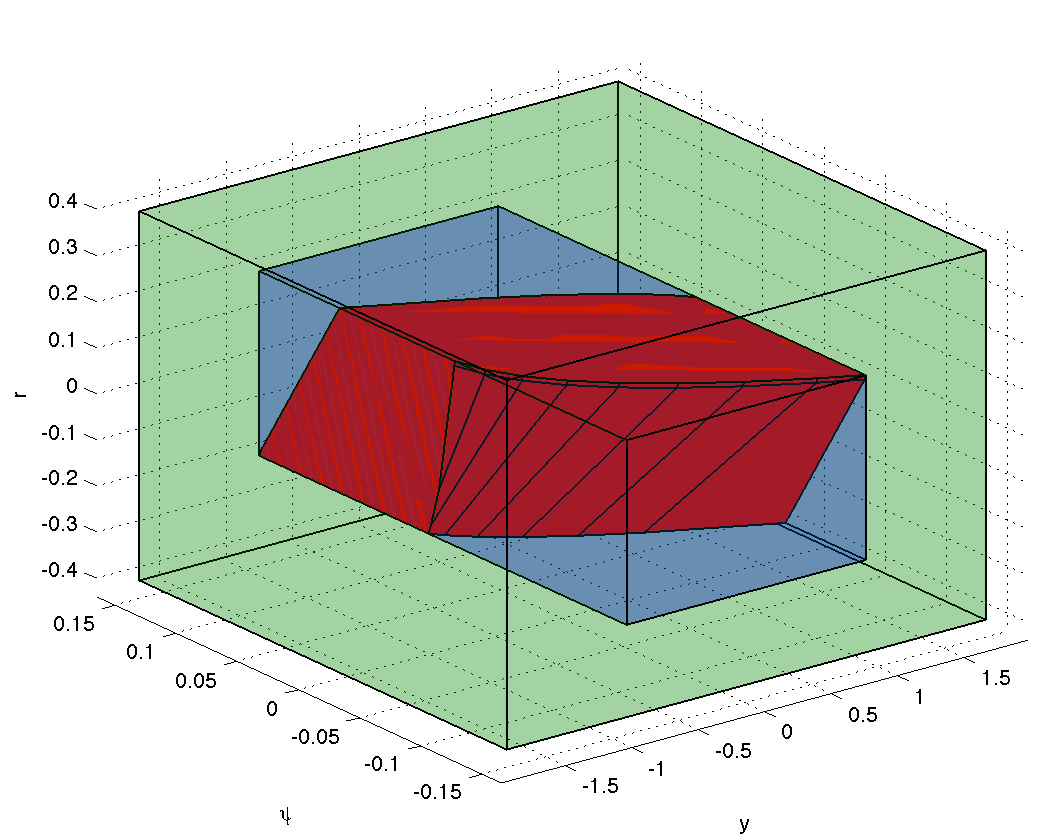
\includegraphics[width=0.4\columnwidth]{invariant}
		% This file was created by matlab2tikz v0.4.7 running on MATLAB 8.2.
% Copyright (c) 2008--2014, Nico Schlömer <nico.schloemer@gmail.com>
% All rights reserved.
% Minimal pgfplots version: 1.3
% 
\begin{tikzpicture}

\begin{axis}[%
width=\figurewidth,
height=\figureheight,
scale only axis,
xmin=0,
xmax=30,
ymin=-0.08,
ymax=0.08,
ylabel={$\delta_f$},
axis x line*=bottom,
axis y line*=left
]
\addplot [color=red,solid,forget plot]
  table[row sep=crcr]{0	0.000743231905265123\\
0.1	0.000743231905265123\\
0.2	0.000700165729183309\\
0.3	0.000679970508631751\\
0.4	0.000671472431817428\\
0.5	0.000642738124028425\\
0.6	0.000520804887834724\\
0.7	0.000462736672700507\\
0.8	0.00047137210619427\\
0.9	0.00028535235777918\\
1	-2.35084338094968e-05\\
1.1	-0.0002275753014195\\
1.2	-0.000311247658226631\\
1.3	-0.000381380334372404\\
1.4	-0.000423959679139044\\
1.5	-0.000420937721875727\\
1.6	-0.000396204349291492\\
1.7	-0.000332280348051709\\
1.8	-0.000276381402053595\\
1.9	-0.00029644535541368\\
2	-0.000470927701123194\\
2.1	-0.00080680470164254\\
2.2	-0.000809783589792539\\
2.3	-0.000717474662874818\\
2.4	-0.000459372524102802\\
2.5	2.12595282748215e-05\\
2.6	0.000121979746719862\\
2.7	3.25318940064762e-05\\
2.8	1.00334579593298e-05\\
2.9	-3.25538190898336e-06\\
3	-6.25214766795208e-06\\
3.1	-4.10043192379571e-06\\
3.2	-1.07599446866335e-07\\
3.3	4.15133382959156e-06\\
3.4	8.03580343591414e-06\\
3.5	1.13279172465667e-05\\
3.6	1.39799584972962e-05\\
3.7	1.60062899981803e-05\\
3.8	1.74431558947431e-05\\
3.9	1.83362343488384e-05\\
4	1.8737510493519e-05\\
4.1	1.87041623035695e-05\\
4.2	1.82971952593421e-05\\
4.3	1.75795282200855e-05\\
4.4	1.66138196513806e-05\\
4.5	1.54603784067037e-05\\
4.6	1.41754001284386e-05\\
4.7	1.28096509295563e-05\\
4.8	1.14076267859245e-05\\
4.9	1.00071556145736e-05\\
5	8.63937432468492e-06\\
5.1	7.32899824338598e-06\\
5.2	6.09479910956921e-06\\
5.3	4.95021509256625e-06\\
5.4	3.90402835725133e-06\\
5.5	2.96105947133031e-06\\
5.6	2.12284157409016e-06\\
5.7	1.38824923616226e-06\\
5.8	7.54067174367577e-07\\
5.9	2.15491669879747e-07\\
6	-2.3343666785431e-07\\
6.1	-5.99466313518614e-07\\
6.2	-8.89829510858017e-07\\
6.3	-1.11199206902224e-06\\
6.4	-1.273451623329e-06\\
6.5	-1.38157782223489e-06\\
6.6	-1.44348826656548e-06\\
6.7	-1.4659546622958e-06\\
6.8	-1.45533426865923e-06\\
6.9	-1.41752242916598e-06\\
7	-1.35792257284061e-06\\
7.1	-1.28143059402366e-06\\
7.2	-1.19243108678314e-06\\
7.3	-1.09480321200438e-06\\
7.4	-9.91934390217209e-07\\
7.5	-8.8674019357339e-07\\
7.6	-7.81689162573842e-07\\
7.7	-6.78831308268801e-07\\
7.8	-5.7982929208434e-07\\
7.9	-4.85991412778851e-07\\
8	-3.98305565662595e-07\\
8.1	-3.17473502611364e-07\\
8.2	-2.4394479223493e-07\\
8.3	-1.77949942405196e-07\\
8.4	-1.19532243882028e-07\\
8.5	-6.85779967582976e-08\\
8.6	-2.48448076365509e-08\\
8.7	1.20122620717554e-08\\
8.8	4.24168276084644e-08\\
8.9	6.68496857284158e-08\\
9	8.58297439431874e-08\\
9.1	9.98973435678736e-08\\
9.2	1.09599909679098e-07\\
9.3	1.15479847401581e-07\\
9.4	1.18064548624598e-07\\
9.5	1.17858367638685e-07\\
9.6	1.15336403189344e-07\\
9.7	1.10939908748702e-07\\
9.8	1.05073149623321e-07\\
9.9	9.81015458065108e-08\\
10	9.03508899719255e-08\\
10.1	8.21075236715971e-08\\
10.2	-0.000699712581403581\\
10.3	-0.00314474145875589\\
10.4	-0.00571097093047445\\
10.5	-0.00495051368065156\\
10.6	-0.00474448508946218\\
10.7	-0.00838464768601333\\
10.8	-0.00902473082722437\\
10.9	-0.00765721615776218\\
11	-0.00960705166111964\\
11.1	-0.017246868557727\\
11.2	-0.0343010945434768\\
11.3	0\\
11.4	-0.0468636648315344\\
11.5	-0.021797107059787\\
11.6	0.0100277617273007\\
11.7	0.0164573118841555\\
11.8	0.0133317238566057\\
11.9	0.00961861531675608\\
12	0.00575802034014757\\
12.1	0.00292743191677348\\
12.2	0.00107554579603402\\
12.3	-0.000143136227779467\\
12.4	0.000426033069931799\\
12.5	0.000583137811913298\\
12.6	-0.000103110800216674\\
12.7	-0.00226217358561809\\
12.8	-0.00579545928299629\\
12.9	-0.00683668139686417\\
13	-0.00487897977682703\\
13.1	-0.00699387840603185\\
13.2	-0.00965568229794052\\
13.3	-0.00726889395410169\\
13.4	-0.00753542938799971\\
13.5	-0.0093162462464131\\
13.6	-0.0157863312218611\\
13.7	-0.0292720072093223\\
13.8	-0.0603096030575979\\
13.9	0\\
14	0.0112919835261615\\
14.1	0.0108854922035298\\
14.2	0.0091077377379632\\
14.3	0.00614016599738922\\
14.4	0.00323465581970863\\
14.5	0.00185469133154417\\
14.6	0.000785048921007491\\
14.7	0.00156046020635403\\
14.8	0.00141159073791819\\
14.9	0.000240802097591361\\
15	-0.00372302886942358\\
15.1	-0.00744792345730491\\
15.2	-0.00616348559889046\\
15.3	-0.00381689209605698\\
15.4	-0.00596961387756183\\
15.5	-0.00703791891530788\\
15.6	-0.00675418287085641\\
15.7	-0.0115189973355846\\
15.8	-0.00694965677426631\\
15.9	-0.00617607413718014\\
16	-0.00894519642735455\\
16.1	-0.0211418090268308\\
16.2	-0.0505331835672633\\
16.3	0\\
16.4	0.00683412027581741\\
16.5	0.00656997557583451\\
16.6	0.0048938399395636\\
16.7	0.00327841159918132\\
16.8	0.00320487999858002\\
16.9	0.00289013075974181\\
17	0.00120929879148058\\
17.1	-0.000137298204397101\\
17.2	-0.00300458610655661\\
17.3	-0.00243654803664765\\
17.4	-0.00443523958442714\\
17.5	-0.00487159632679648\\
17.6	-0.00481325198253085\\
17.7	-0.0057808794534245\\
17.8	-0.00785084657084628\\
17.9	-0.00750017986169255\\
18	-0.0117386326966227\\
18.1	-0.0242468272573219\\
18.2	-0.045037099815463\\
18.3	0\\
18.4	0.00533043845527063\\
18.5	0.00698671474776983\\
18.6	0.00512633301758456\\
18.7	0.00377629379005456\\
18.8	0.00278900662053001\\
18.9	0.00109662838832064\\
19	2.25981202197859e-05\\
19.1	-0.00232880359364243\\
19.2	-0.00274321950523067\\
19.3	-0.00863238693558017\\
19.4	-0.00521755523267533\\
19.5	-0.00568656665757681\\
19.6	-0.0106722116731533\\
19.7	-0.00784269433737462\\
19.8	-0.0106884047669077\\
19.9	-0.0071681282130564\\
20	-0.00490650710996029\\
20.1	-0.00295406440497855\\
20.2	-0.00123760153912038\\
20.3	0.00196806897651989\\
20.4	0.00464407799152508\\
20.5	0.00370874181277834\\
20.6	0.00446147483318526\\
20.7	0.00537407315092352\\
20.8	0.0074221444280703\\
20.9	0.00987992742024953\\
21	0.0107811942031612\\
21.1	0.0112631973698815\\
21.2	0.0130815639334085\\
21.3	0.0163897421116388\\
21.4	0.0163035450723334\\
21.5	0.0189975890424526\\
21.6	0.0251786148364771\\
21.7	0.0325654782695197\\
21.8	0.0181020033289579\\
21.9	-0.0113103576343168\\
22	-0.0132052265925594\\
22.1	-0.0116064756971495\\
22.2	-0.00781829333920731\\
22.3	-0.00502967305569405\\
22.4	-0.0010614539055855\\
22.5	-0.000182564655144391\\
22.6	-0.000218314243327326\\
22.7	-0.000209945857307397\\
22.8	0.00101168955237632\\
22.9	0.00249459210535268\\
23	0.00438371074279337\\
23.1	0.00588981854192593\\
23.2	0.0078788255378834\\
23.3	0.00775174543538604\\
23.4	0.00984678377224535\\
23.5	0.00979588801450992\\
23.6	0.0140478561167377\\
23.7	0.024580167539114\\
23.8	0.0412274836977117\\
23.9	0\\
24	-0.00598100410683227\\
24.1	-0.00550647867746145\\
24.2	-0.00641660226841587\\
24.3	-0.00409038950365503\\
24.4	-0.00065007765234712\\
24.5	-0.00190237573873934\\
24.6	-0.00107526732779661\\
24.7	0.000666994387542494\\
24.8	0.00176687581938799\\
24.9	0.00399860136852886\\
25	0.00572995210282142\\
25.1	0.00795431279514382\\
25.2	0.00723197864436481\\
25.3	0.0087220344281176\\
25.4	0.0114294990525708\\
25.5	0.0204956216454751\\
25.6	0.0379371601198503\\
25.7	0\\
25.8	-0.00374220830879278\\
25.9	-0.0035669165629135\\
26	-0.00461044358185793\\
26.1	-0.00390434295471776\\
26.2	-0.00334855263396799\\
26.3	-0.000770040506197288\\
26.4	0.00102333394913526\\
26.5	0.00320579464479902\\
26.6	0.00449046439777033\\
26.7	0.00596865156675076\\
26.8	0.00893746713748292\\
26.9	0.00710694178874824\\
27	0.00760574555421061\\
27.1	0.0135325003855458\\
27.2	0.0287314858570169\\
27.3	0.0617510910299495\\
27.4	0.0400892446910649\\
27.5	-0.0141405676660801\\
27.6	0\\
27.7	-0.0276816613108126\\
27.8	-0.0286486955979465\\
27.9	-0.0192721871587083\\
28	-0.0116463227196317\\
28.1	-0.00346026536868545\\
28.2	0.000257693157179542\\
28.3	0.0019969735145004\\
28.4	0.00234526077857976\\
28.5	0.00190953002612277\\
28.6	0.00204244709549416\\
28.7	0.00318276060045973\\
28.8	0.00399852331950978\\
28.9	0.00615625261292781\\
29	0.00822283762850023\\
29.1	0.00886032001560287\\
29.2	0.0131734890341103\\
29.3	0.0131579602678317\\
29.4	0.0112068436136657\\
29.5	0.0142322192918644\\
29.6	0.0205673326586579\\
29.7	0.032148019235408\\
29.8	0.0496400091556592\\
29.9	-0.00349713936768268\\
30	-0.0134370966977978\\
};
\end{axis}
\end{tikzpicture}%
	\end{center}
	\caption{Input: steering angle.}
	\label{fig:df}
\end{figure}
% section simulation (end)

\end{document}